\documentclass[10pt]{beamer}
\usetheme[
%%% options passed to the outer theme
%    hidetitle,           % hide the (short) title in the sidebar
%    hideauthor,          % hide the (short) author in the sidebar
%    hideinstitute,       % hide the (short) institute in the bottom of the sidebar
%    shownavsym,          % show the navigation symbols
%    width=2cm,           % width of the sidebar (default is 2 cm)
%    hideothersubsections,% hide all subsections but the subsections in the current section
%    hideallsubsections,  % hide all subsections
    left,               % right of left position of sidebar (default is right)
%%% options passed to the color theme
%    lightheaderbg,       % use a light header background
  ]{AAUsidebar}

% If you want to change the colors of the various elements in the theme, edit and uncomment the following lines
% Change the bar and sidebar colors:
%\setbeamercolor{AAUsidebar}{fg=red!20,bg=red}
%\setbeamercolor{sidebar}{bg=red!20}
% Change the color of the structural elements:
%\setbeamercolor{structure}{fg=red}
% Change the frame title text color:
%\setbeamercolor{frametitle}{fg=blue}
% Change the normal text color background:
%\setbeamercolor{normal text}{bg=gray!10}
% ... and you can of course change a lot more - see the beamer user manual.


\usepackage[utf8]{inputenc}
\usepackage[english]{babel}
\usepackage[T1]{fontenc}
\usepackage{multimedia}
\usepackage{graphicx} % enable fitting figures
\usepackage{wrapfig}
\usepackage{adjustbox}
% Or whatever. Note that the encoding and the font should match. If T1
% does not look nice, try deleting the line with the fontenc.
\usepackage{helvet}
\usepackage{tikz}
\usetikzlibrary{shapes,shapes.geometric, arrows,positioning,calc}
\tikzset{
	block/.style = {draw, fill=white, rectangle, minimum height=3em, minimum width=3em},
	tmp/.style  = {coordinate}, 
	sum/.style= {draw, fill=white, circle, node distance=1cm},
	input/.style = {coordinate},
	output/.style= {coordinate},
	pinstyle/.style = {pin edge={to-,thin,black}
	}
}

\usepackage{amsmath}
\usepackage{amssymb}
\usepackage{kbordermatrix}

% colored hyperlinks
\newcommand{\chref}[2]{%
  \href{#1}{{\usebeamercolor[bg]{AAUsidebar}#2}}%
}

\title[Modelling and Networked Control of Water Distribution Networks]% optional, use only with long paper titles
{Multivariable Control of A Reefer Trailer}

% \subtitle{}  % could also be a conference name

\date{\today}

\author[CA834] % optional, use only with lots of authors
{
  CA834
}
% - Give the names in the same order as they appear in the paper.
% - Use the \inst{?} command only if the authors have different
%   affiliation. See the beamer manual for an example

\institute[
%  {\includegraphics[scale=0.2]{aau_segl}}\\ %insert a company, department or university logo
  Control and Automation\\
  Aalborg University\\
  Denmark
] % optional - is placed in the bottom of the sidebar on every slide
{% is placed on the title page
  Control and Automation, Group 834\\
  Aalborg University\\
  Denmark
  
  %there must be an empty line above this line - otherwise some unwanted space is added between the university and the country (I do not know why;( )
}


% specify a logo on the titlepage (you can specify additional logos an include them in 
% institute command below
\pgfdeclareimage[height=1.5cm]{titlepagelogo}{AAUgraphics/aau_logo_new} % placed on the title page
%\pgfdeclareimage[height=1.5cm]{titlepagelogo2}{graphics/aau_logo_new} % placed on the title page
\titlegraphic{% is placed on the bottom of the title page
  \pgfuseimage{titlepagelogo}
%  \hspace{1cm}\pgfuseimage{titlepagelogo2}
}


\begin{document}
% the titlepage
{\aauwavesbg%
\begin{frame}[plain,noframenumbering] % the plain option removes the sidebar and header from the title page
  \titlepage
\end{frame}}


%%%%%%%%%%%%%%%%

% TOC
\begin{frame}{Agenda}{}
\tableofcontents
\end{frame}






% ======================================================================
% Inputs for topics here!

\section{Introduction}
\begin{frame}{Introduction}{What is a Reefer Trailer}
 		\begin{columns}
 		\begin{column}{.5\textwidth}
 			\textbf{Reefer trailer}
	 			\begin{itemize}
		 			\item Transport of perishable goods
		 			\item On land, via trucks
		 			\item Self supplying, batteries			
		 		\end{itemize} \bigskip\bigskip
 			\textbf{Role} 
		 		\begin{itemize}
		 			\item Critical link in global logistics
		 			\item Extends durability of cargo
		 			\item To and from distribution centers			
		 		\end{itemize}
 		\end{column}
 		\begin{column}{.5\textwidth}
 				\raggedleft
 				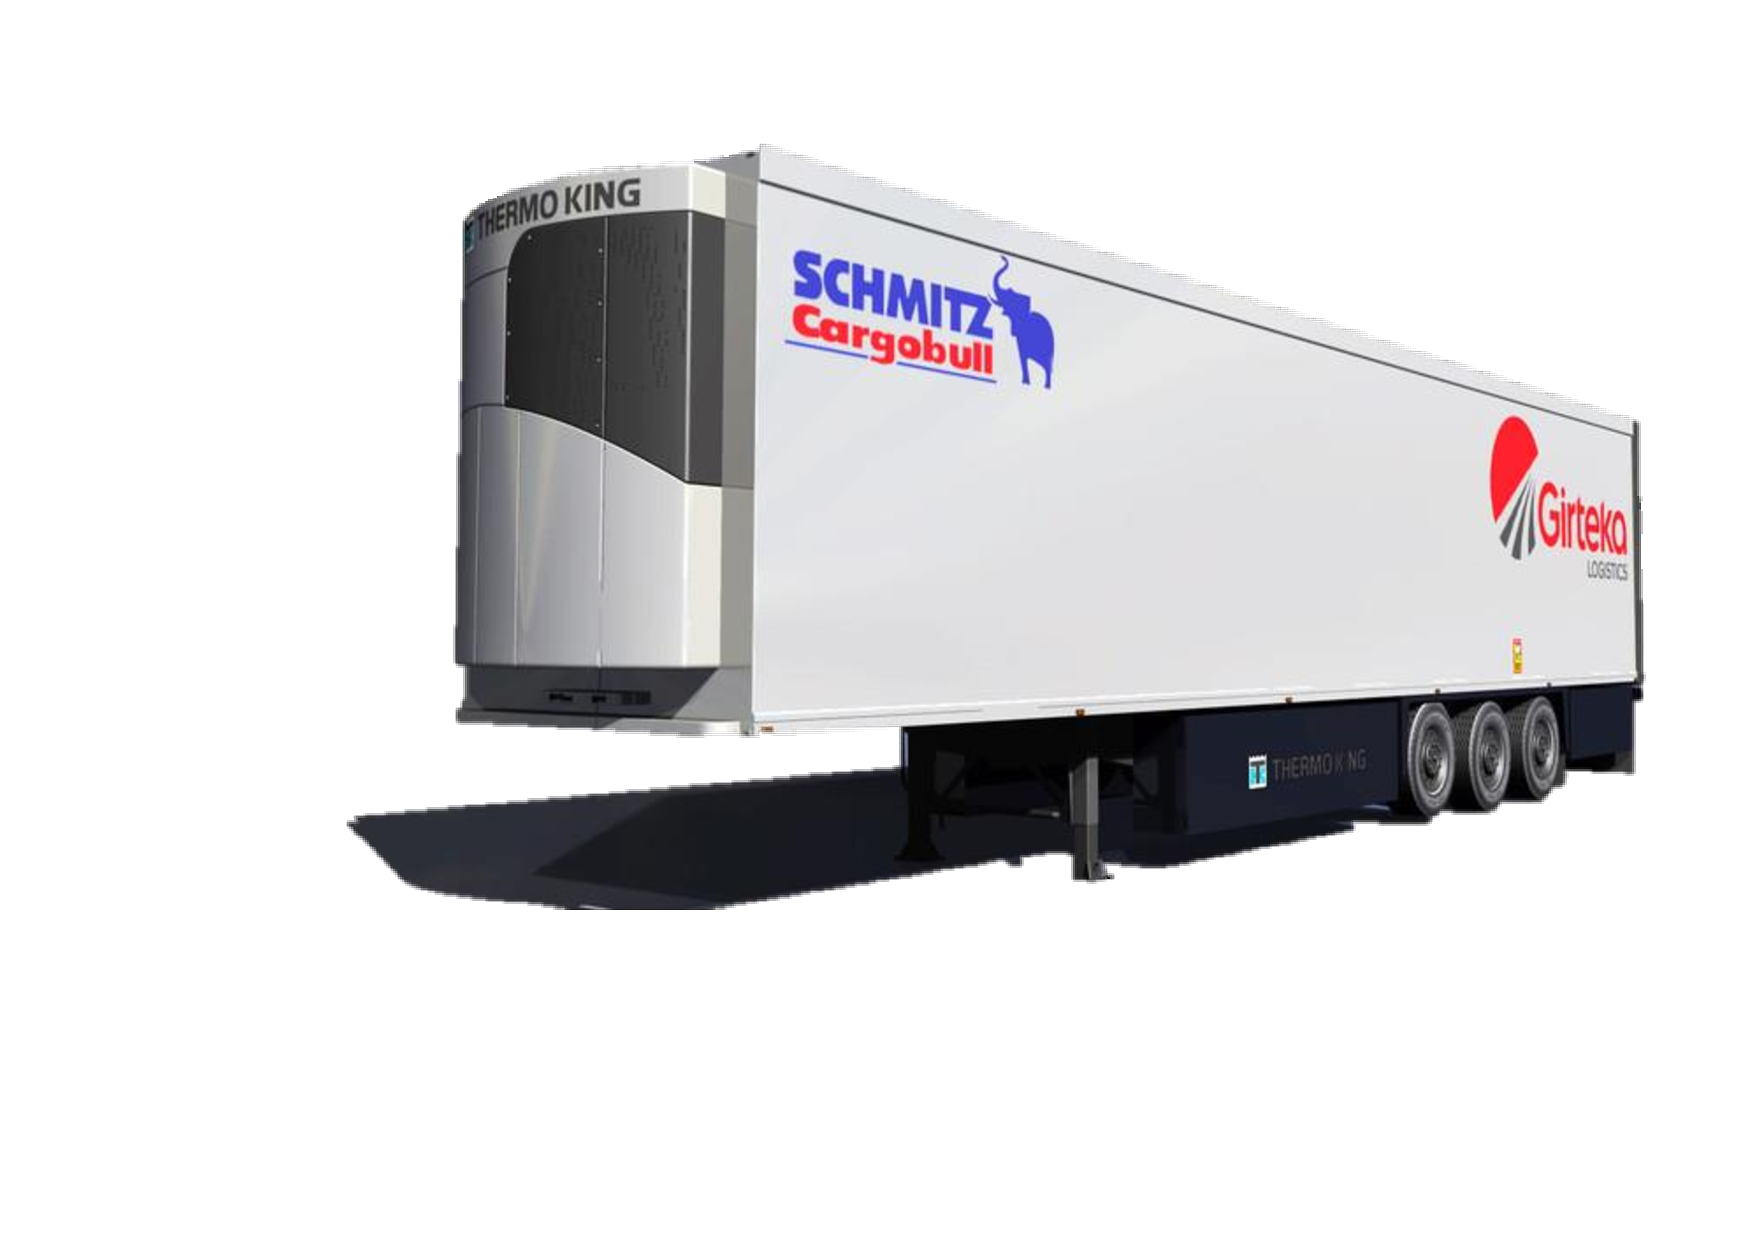
\includegraphics[width=.95\textwidth]{../Graphics/3d_draw_trailer.pdf}
				\centering
				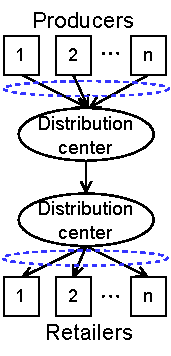
\includegraphics[width=0.45\textwidth]{../Graphics/Transportation_networks.pdf}
 		\end{column}
 	\end{columns}	
\end{frame}

%%%%%%%%%%%%%%%%

\begin{frame}{Introduction}{Efficiency Motivation}
	\begin{itemize}
		\item Increased energy efficiency $\rightarrow$ less power required $\rightarrow$ reduced operational costs  
		\item Smaller batteries $\rightarrow$ reduced capital costs		
	\end{itemize}\bigskip
	\textbf{Efficiency of Reefer Trailers: UN's Sustainable Development Goals}
	\begin{itemize}	
		\item 2nd: Food supply
		\begin{itemize}
			\item Cost of fresh food is correlated with transport costs
			\item Reduced costs increase access to fresh foods for low income people		
		\end{itemize}
		\item 7th: Energy efficiency
		\begin{itemize}
			\item Decreased CO2 emissions per transported good
			\item Decreased use of rare metals for batteries	
		\end{itemize}
	\end{itemize}	
\end{frame}

%%%%%%%%%%%%%%%%%
\begin{frame}{Introduction}{Concept of Reefer trailer}
%	\textbf{Some text}
	\begin{itemize}
		\item Insulated trailer
		\item Heat need be removed from cargo through airflow	
	\end{itemize}
	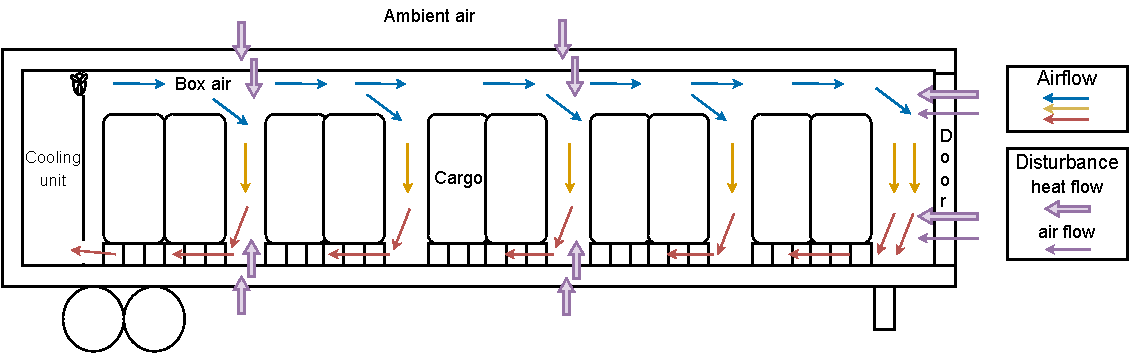
\includegraphics[width=1\textwidth]{../Graphics/Trailer_airflow.pdf}
	\begin{itemize}
		\item High-Fidelity (Hi-Fi) simulation model of trailer is supplied by BITZER
		\item Hi-Fi model is implemented with PID controllers
	\end{itemize}
\end{frame}

%%%%%%%%%%%%%%%%%
\begin{frame}{Introduction}{Problem Definition}
	\textbf{Problem Definition:} Can a MIMO controller be designed to improve energy efficiency of the reefer trailer Hi-Fi simulation model?
	\begin{itemize}
		\item Boiled down a bit. 
		\item Stable MIMO controller
	\end{itemize}
\end{frame}

%%%%%%%%%%%%%%%%%
\begin{frame}{System Description}{Refrigeration circuit}
	\textbf{Two stage refrigeration system with flash tank}
	\begin{itemize}
		\item Increased efficiency compared to one stage system 
		\item Subcooling throttle is not modeled
		\item Controlled inputs and outputs
		\begin{itemize}
			\item 5 inputs, 2 outputs
		\end{itemize}
		\item Load delivers heat to evaporator
	\end{itemize}
\begin{figure}[h]
	\centering
	\begin{minipage}{0.6\textwidth}
		\centering
		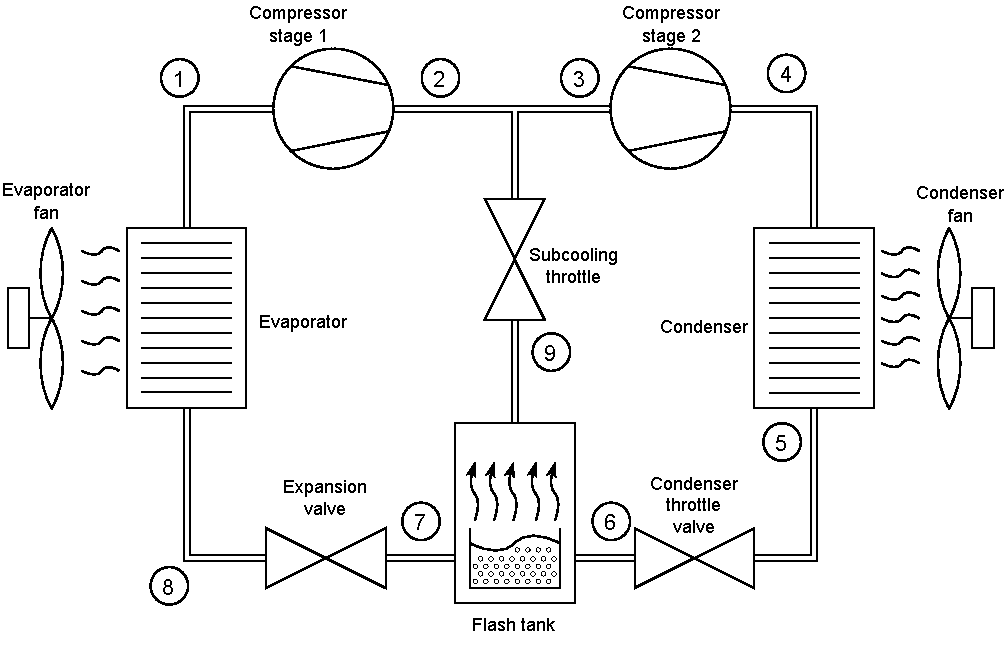
\includegraphics[width=1\textwidth]{../Graphics/HVAC_Diagram_Fans.pdf} % first figure itself
%		\caption{Illustration of two stage refrigeration circuit}
%		\label{fig:HVAC_Diagram}
	\end{minipage}\hfill
	\begin{minipage}{0.4\textwidth}
		\centering
		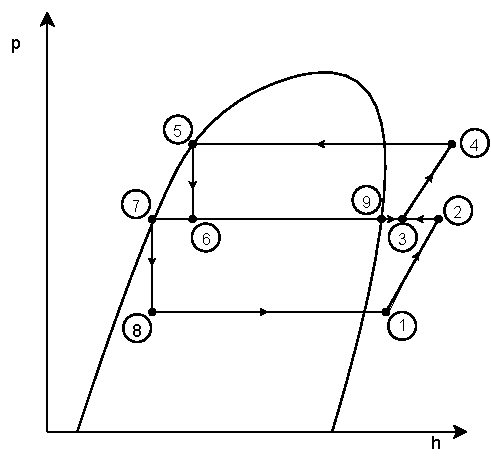
\includegraphics[width=1.05\textwidth]{../Graphics/Flash_Tank_P-h_Diagram} % second figure itself
%		\caption{Illustration of p-h diagram of two stage refrigeration circuit}
%		\label{fig:p-h_diagram}
	\end{minipage}
\end{figure}
\end{frame}

%%%%%%%%%%%%%%%%%
%\begin{frame}{System description}{Entire System}
%	
%	\textbf{Some text}
%	\begin{itemize}
%		\item Item
%	\end{itemize}
%\end{frame}

%%%%%%%%%%%%%%%%%%
%\begin{frame}{System description}{}
%	\textbf{Some text}
%	\begin{itemize}
%		\item Item
%	\end{itemize}
%\end{frame}
%
%%%%%%%%%%%%%%%%%%
%\begin{frame}{System description}{}
%	\textbf{Some text}
%	\begin{itemize}
%		\item Item
%	\end{itemize}
%\end{frame}

%%%%%%%%%%%%%%%%%%
%\begin{frame}{Next slide title}{Next slide subtitle}
%	\textbf{Some text}
%	\begin{itemize}
%		\item Item
%	\end{itemize}
%\end{frame}
%
%%%%%%%%%%%%%%%%%%
%\begin{frame}{Next slide title}{Next slide subtitle}
%	\textbf{Some text}
%	\begin{itemize}
%		\item Item
%	\end{itemize}
%\end{frame}
%
%%%%%%%%%%%%%%%%%%
%\begin{frame}{Next slide title}{Next slide subtitle}
%	\textbf{Some text}
%	\begin{itemize}
%		\item Item
%	\end{itemize}
%\end{frame}
%
%%%%%%%%%%%%%%%%%%

\section{Modeling}
\begin{frame}{Modelling}{Introduction}
	First principles model derived, linearised and further developed for observer based control.
	\begin{itemize}
		\item \textbf{Main goal:} Capture dynamics important for the box air temperature (main control objective)
		\begin{itemize}
			\item Thermal masses: Trailer box, cargo, evaporator, condenser.
		\end{itemize}
		\item \textbf{Modular approach:} Inputs, outputs, internal equations/states
		\item \textbf{Slow vs. fast dynamics:} States or algebraic equations
		\begin{itemize}
			\item Including faster dynamics = more accurate model
			\item Unnecessary from control perspective.
		\end{itemize}	
		\item All energy balances are defined in steady-state (SS)
	\end{itemize}
\end{frame}



%%%%%%%%%%%%%%%%%

\begin{frame}{Modelling}{Component Models}
	Each component is modelled separately. The components are:
	\begin{itemize}
		\item Expansion Valve
		\item Pipe joining junction
		\item Compressor
		\item Condenser
		\item Flash tank
		\item Evaporator
		\item Box
	\end{itemize}
	
	Only the most relevant components and equations are included in the following.
\end{frame}



%%%%%%%%%%%%%%%%%

\begin{frame}{Modelling}{Expansion Valve}
	\textbf{Purpose:} Lower pressure of liquid refrigerant from flash tank to evaporator.
	\begin{itemize}
		\item Adiabatic process: Modelled algebraicly
	\end{itemize}
	Flow through valve:
	\begin{equation} \label{eq:ExpansionValve_Alt}
		\begin{split}
			\dot{m} & = f_p(\Theta) K  \sqrt{\frac{1}{v_{in}} (p_{in} - p_{out})} \\
		\end{split}
	\end{equation}

\end{frame}



%%%%%%%%%%%%%%%%%

\begin{frame}{Modelling}{Compressor}
	\textbf{Purpose:} Generate pressure sufficient for refrigerant flow and condenser heat flow to ambient air.
	\begin{itemize}
		\item Two compressor stages
		\item Modelled as reciprocating (piston) compressor
		\item Modelled algebraicly - Fast dynamics do not affect slow evaporator dynamics
	\end{itemize}
	Flow through compressor:
	\begin{equation}
		\dot{m} = \left(\frac{V_1}{v_1} - \frac{V_C}{v_2}\right) \frac{\omega}{2} \label{eq:comp_mass_flow}
	\end{equation}
\end{frame}

%%%%%%%%%%%%%%%%%

\begin{frame}{Modelling}{Condenser}
	\textbf{Purpose:} Exchange heat from hot vapour refrigerant to outside ambient air.
	\begin{itemize}
		\item Modelled as one control volume (CV)
		\item States: $M_r$ and $T_m$
	\end{itemize}
	\begin{figure}[h!]
		\centering
		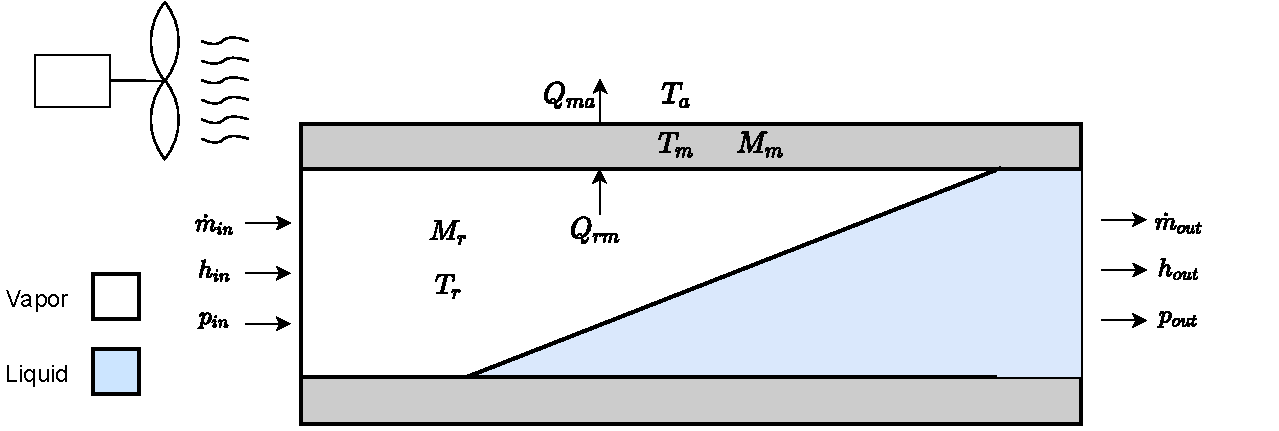
\includegraphics[width=1\textwidth]{../Graphics/Condenser.pdf}
		\caption{Diagram of condenser control volume}
		\label{fig:condenser_CV}
	\end{figure}
\end{frame}
\begin{frame}{Condenser}{Equations}
	Energy balance:
	\begin{equation}
		h_{out} = h_{in} - \frac{Q_{rm}}{\dot{m}_{in}} \label{eq:Condenser_Enthalpy}
	\end{equation}
	Refrigerant mass balance:
	\begin{equation}
		\frac{dM_r}{dt} 	 = \dot{m}_{in}(t) - \dot{m}_{out}(t) \label{eq:Condenser_ChangeOfMass}
	\end{equation}
	Metal energy balance:
	\begin{equation}
		\frac{dT_m}{dt} 	 = \frac{Q_{rm} - Q_{ma}}{M_m \cdot Cp_m} \label{eq:Condenser_ChangeOfTemperature}
	\end{equation}
\end{frame}




%%%%%%%%%%%%%%%%%

\begin{frame}{Modelling}{Evaporator}
	\textbf{Purpose:} Exchange heat from box air to cold liquid refrigerant.
	\begin{itemize}
		\item Superheat is important control objective
		\item Modelled with two CVs: liquid-vapour and vapour separated by $\sigma$
		\item Simplification: Pressure out = in
		\item States: $T_{mlv}$, $T_{mv}$, $M_{lv}$, $M_{v}$ and $T_{v}$
	\end{itemize}
	
	\vspace{0.4cm}
	\begin{figure}[h!]
		\centering
		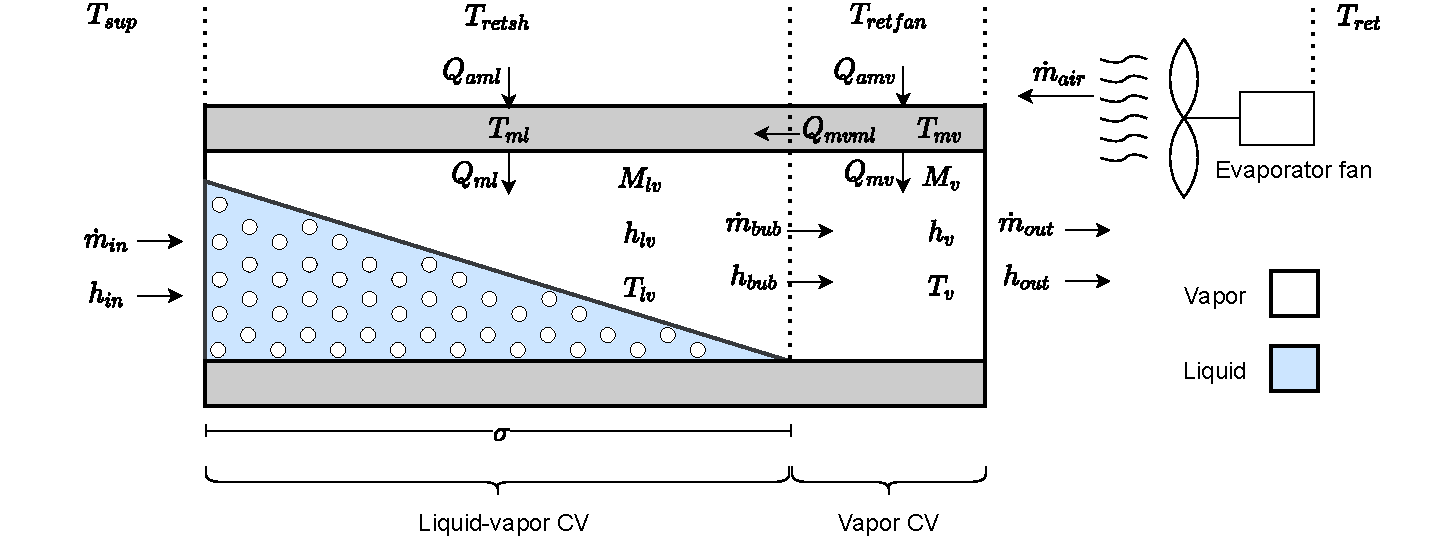
\includegraphics[width=1\textwidth]{../Graphics/Evaporator_CV_diagram.pdf}
		\label{fig:evap_CV}
	\end{figure}

\end{frame}

\begin{frame}{Evaporator}{Equations}
	Moving boundary:
	\begin{equation}
		\sigma = \frac{M_{lv} \cdot v_{lv}}{V_i} \label{eq:Evaporator_boundary}
	\end{equation}
	Liquid-vapour CV metal energy balance:
	\begin{equation}
		\frac{dT_{mlv}}{dt}  = \frac{Q_{amlv}-Q_{mlv} + Q_{mvmlv}}{M_m \cdot \sigma \cdot Cp_m} \label{eq:evap_dT_ml}
	\end{equation}
	Vapour CV metal energy balance:
	\begin{equation}
		\frac{dT_{mv}}{dt} = \frac{Q_{amv} - Q_{mv} - Q_{mvmlv}}{M_m \cdot (1 - \sigma) \cdot Cp_m} \label{eq:evap_dT_mv}
	\end{equation}
	Refrigerant mass balances:
	\begin{equation} \label{eq:evap_dMlv}
		\frac{dM_{lv}}{dt} = \dot{m}_{in} - \dot{m}_{dew} \hspace{0.8cm}  \frac{dM_v}{dt} = \dot{m}_{dew} - \dot{m}_{out}
	\end{equation}
	Vapour refrigerant (output) temperature:
	\begin{equation}\label{eq:tv_initial}
		\frac{dT_{v}}{dt} = \bar{T_v} - T_v
	\end{equation}

\end{frame}

%%%%%%%%%%%%%%%%%

\begin{frame}{Modelling}{Box}
	\textbf{Purpose:} Isolate cargo from ambient air and allow for air circulation.
	\begin{itemize}
		\item Contains greatest thermal masses: Box and Cargo
		\item Cargo coupled to air due to large cargo surface area
		\item States: $T_{air}$, $T_{box}$ and $T_{cargo}$
	\end{itemize}
	\begin{figure}[h!]
		\centering
		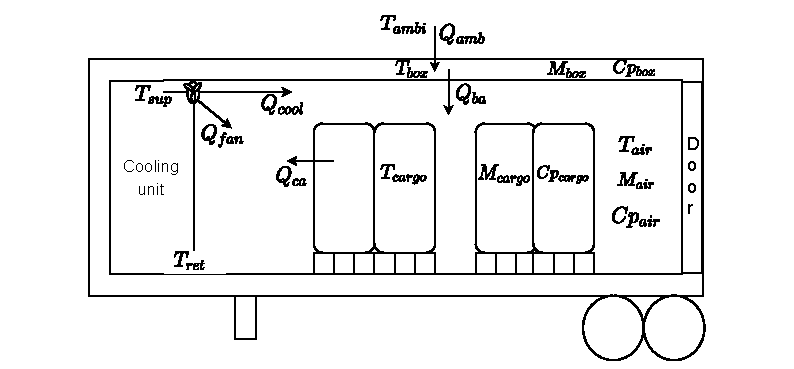
\includegraphics[width=0.8\textwidth]{../Graphics/Box.pdf}
		\caption{Simplified diagram of trailer box}
		\label{fig:box_diagram}
	\end{figure}


\end{frame}

\begin{frame}{Box}{Equations}
	Air, box and cargo energy balances:
	\begin{align}
		\frac{dT_{air}}{dt} &= \frac{Q_{ca} + Q_{ba} + Q_{fan} -Q_{cool}}{M_{air} \cdot Cp_{air}} \label{eq:box_dT_air} \\
		\frac{dT_{box}}{dt} &= \frac{Q_{amb} - Q_{ba}}{M_{box} \cdot Cp_{box}} \label{eq:box_dT_box} \\
		\frac{dT_{cargo}}{dt} &= \frac{-Q_{ca}}{M_{cargo} \cdot Cp_{cargo}} \label{eq:box_dT_cargo}
	\end{align}
	Heat flows:
	\begin{align}
		Q_{cool}   & = Cp_{air} \cdot \dot{m}_{air} \cdot (T_{ret} - T_{sup})	\label{eq:box_Qcool} \\
		Q_{amb}    & = (T_{ambi} - T_{box}) \cdot U A_{amb}						\label{eq:box_Qab}   \\
		Q_{ba}     & = (T_{box} - T_{air}) \cdot U A_{ba}						\label{eq:box_Qba}   \\
		Q_{ca}     & = (T_{cargo} - T_{air}) \cdot U A_{ca}                  	\label{eq:box_Qca}
	\end{align}
\end{frame}



%%%%%%%%%%%%%%%%%

\begin{frame}{Modelling}{Component Input/Output relationship}
	\begin{itemize}
		\item \color{red} Red \color{black}: Missing outputs - Steady-state (SS) values from Hi-Fi simulation
		\item \color{blue} Blue \color{black}: Unused outputs of components
	\end{itemize}
	\begin{figure}[h!]
		\centering
		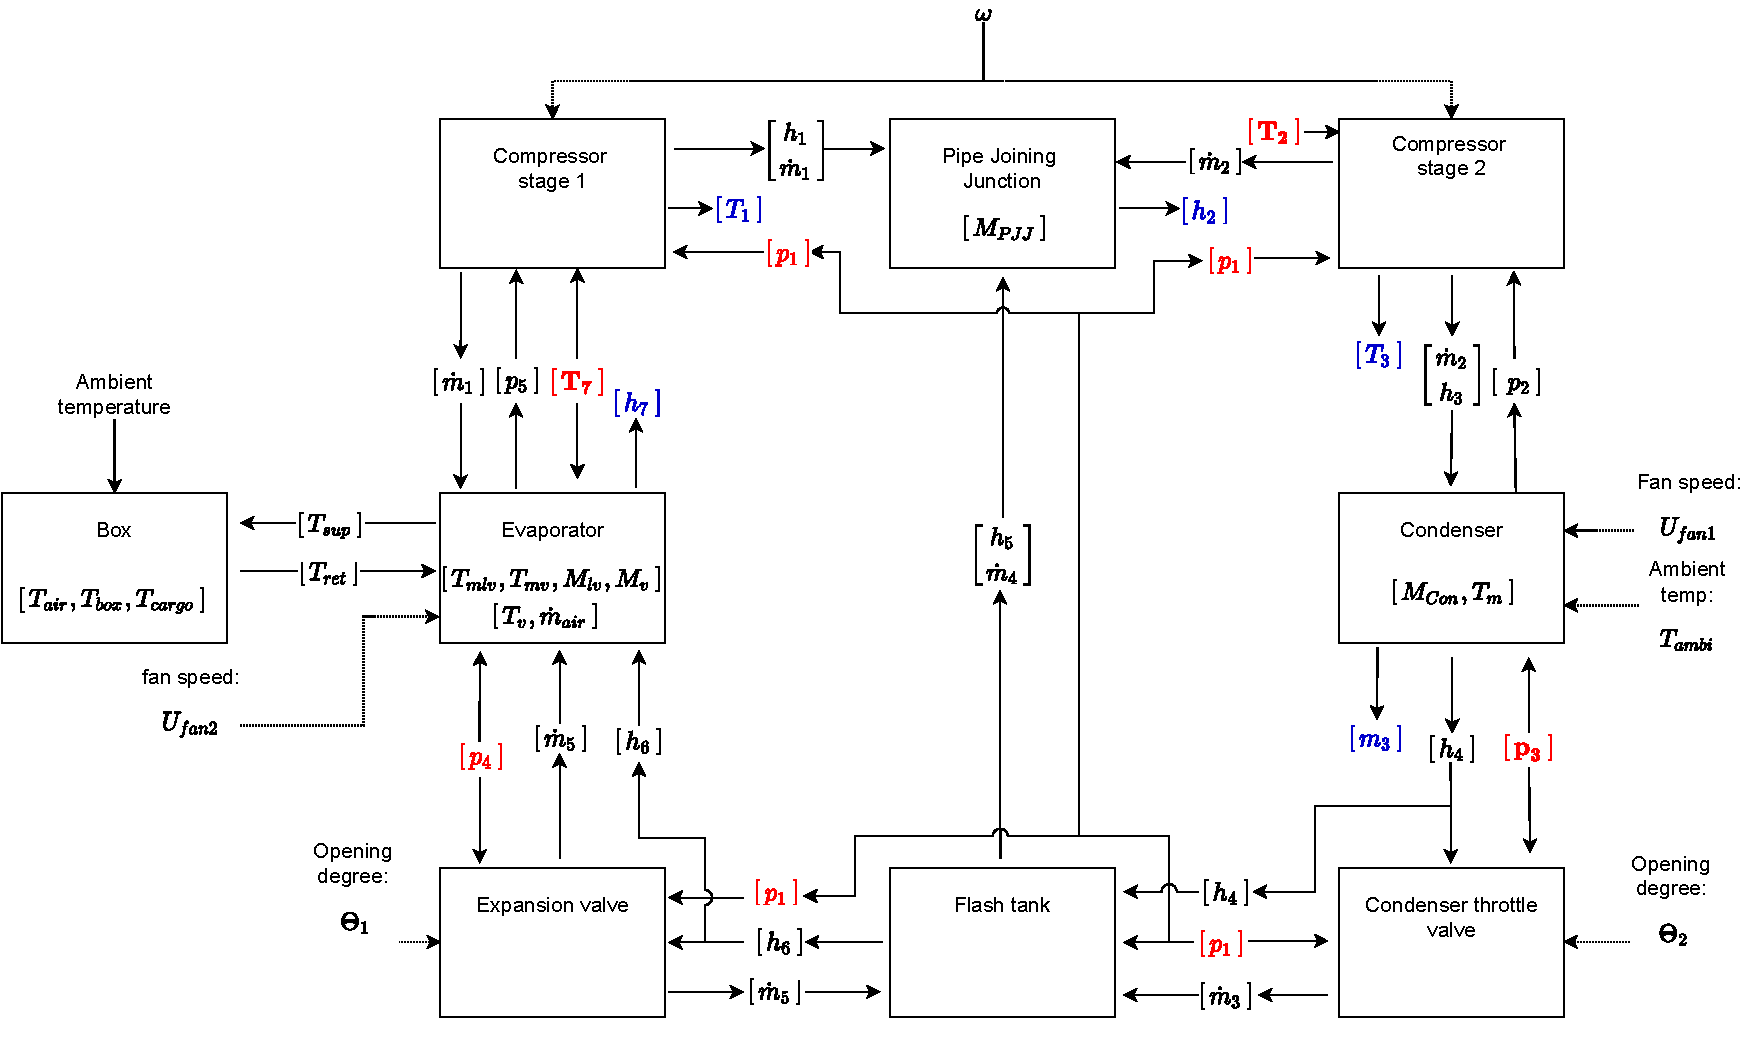
\includegraphics[width=1.04\textwidth]{../Graphics/Block_Diagram_inout_flowValveVersion.pdf}
		\label{fig:Block_diagram_inout}
	\end{figure}
	
\end{frame}

%%%%%%%%%%%%%%%%%

\begin{frame}{Modelling}{Component Input/Output relationship}
	\begin{itemize}
		\item All table lookups are SS variables at operating point (OP)
			\begin{itemize}
				\item Reduces complexity and eases linearisation
				\item Downside: Removes dependencies between states and inputs
			\end{itemize}
	\end{itemize}
\end{frame}




%%%%%%%%%%%%%%%%%

\begin{frame}{Modelling}{Formulating non-linear state-space model}
	A non-linear state space model is formulated
	\begin{itemize}
		\item State equations are collected in a $f(x,u,d)$ vector
		\item Algebraic equations are constraints
	\end{itemize}

	The state, input and disturbance vector are:
	\begin{equation}  \label{eq:xu}
		\begin{split}
			x & = [M_{pjj}	\;
				M_{con} \;
				T_m \;
				\dot{m}_{air}\;
				T_{mlv}      \;
				T_{mv}       \;
				M_{lv}       \;
				M_v          \;
				T_{air}      \;
				T_{box}      \;
				T_{cargo}    \;
				T_v]^T \\
			u & = [\omega	\;
				\Theta_1	\;
				\Theta_2     \;
				U_{fan_1}    \;
				U_{fan_2}]^T \\
			d & = [T_{ambi}]
		\end{split}
	\end{equation}
	System contains 12 states - a lot less than previous work.

\end{frame}



%%%%%%%%%%%%%%%%%

\begin{frame}{Modelling}{Non-linear state-space system}
	The resulting non-linear states-space system becomes:
	\begin{figure}[h!]
		\centering
		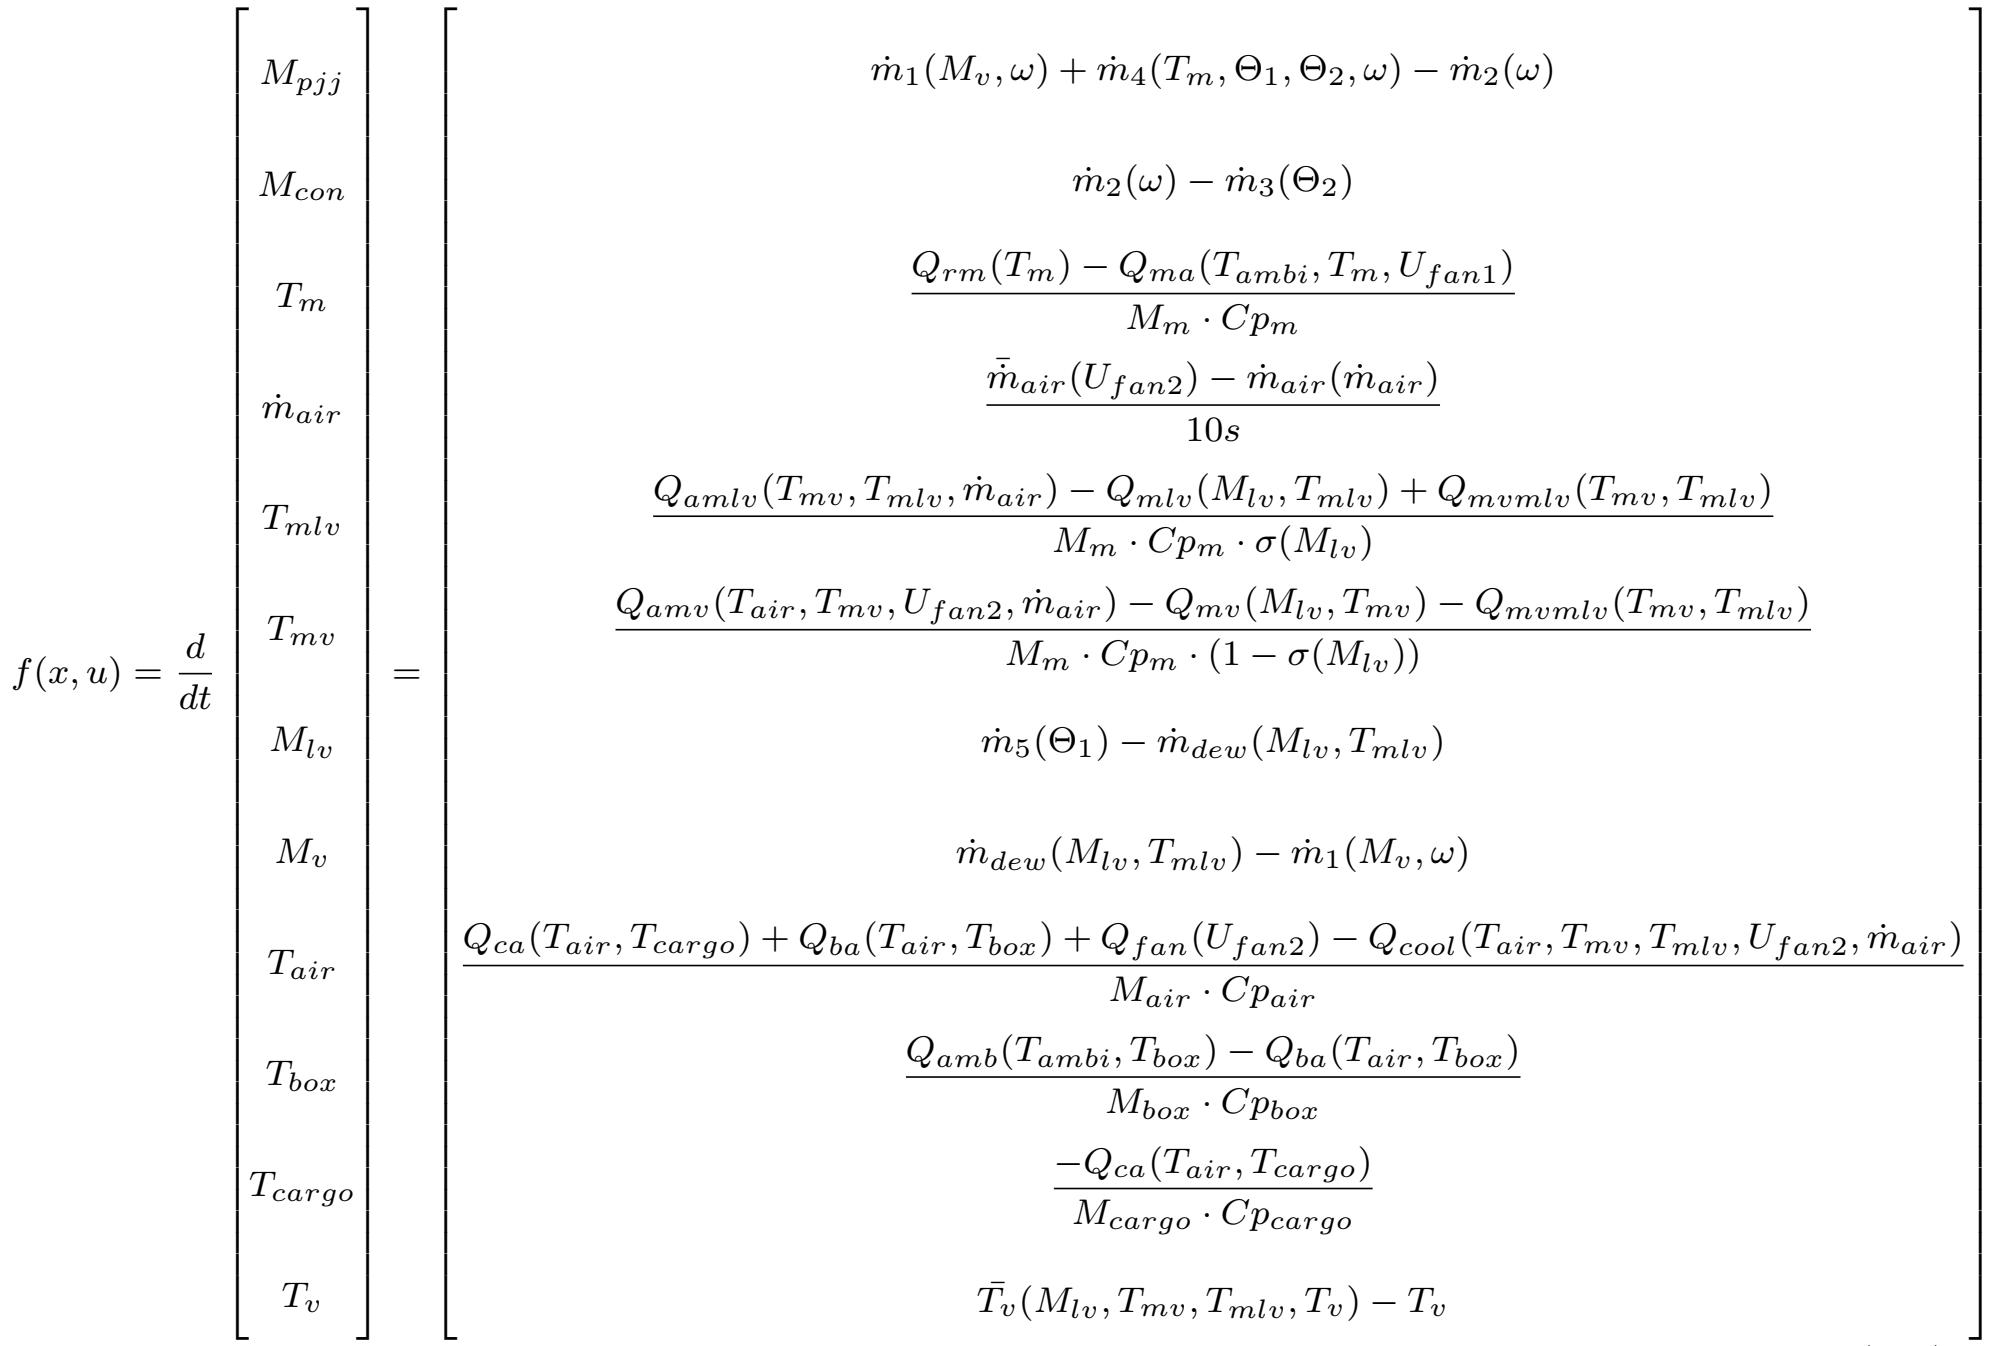
\includegraphics[width=1.04\textwidth]{Graphics/f_x_u.jpeg}
		\label{fig:f_x_u}
	\end{figure}
\end{frame}





%%%%%%%%%%%%%%%%%

\begin{frame}{Modelling}{Verification}
	\begin{itemize}
		\item Model is verified with simulation
		\item Simulated at OP derived from Hi-Fi simulation
		\item 'Faulty' states: $M_{pjj}$ and $M_{Con}$ with constant derivatives
		\begin{itemize}
			\item Not affecting other states $\rightarrow$ Removed
		\end{itemize}
	\end{itemize}
	\begin{figure}[h]
		\centering
		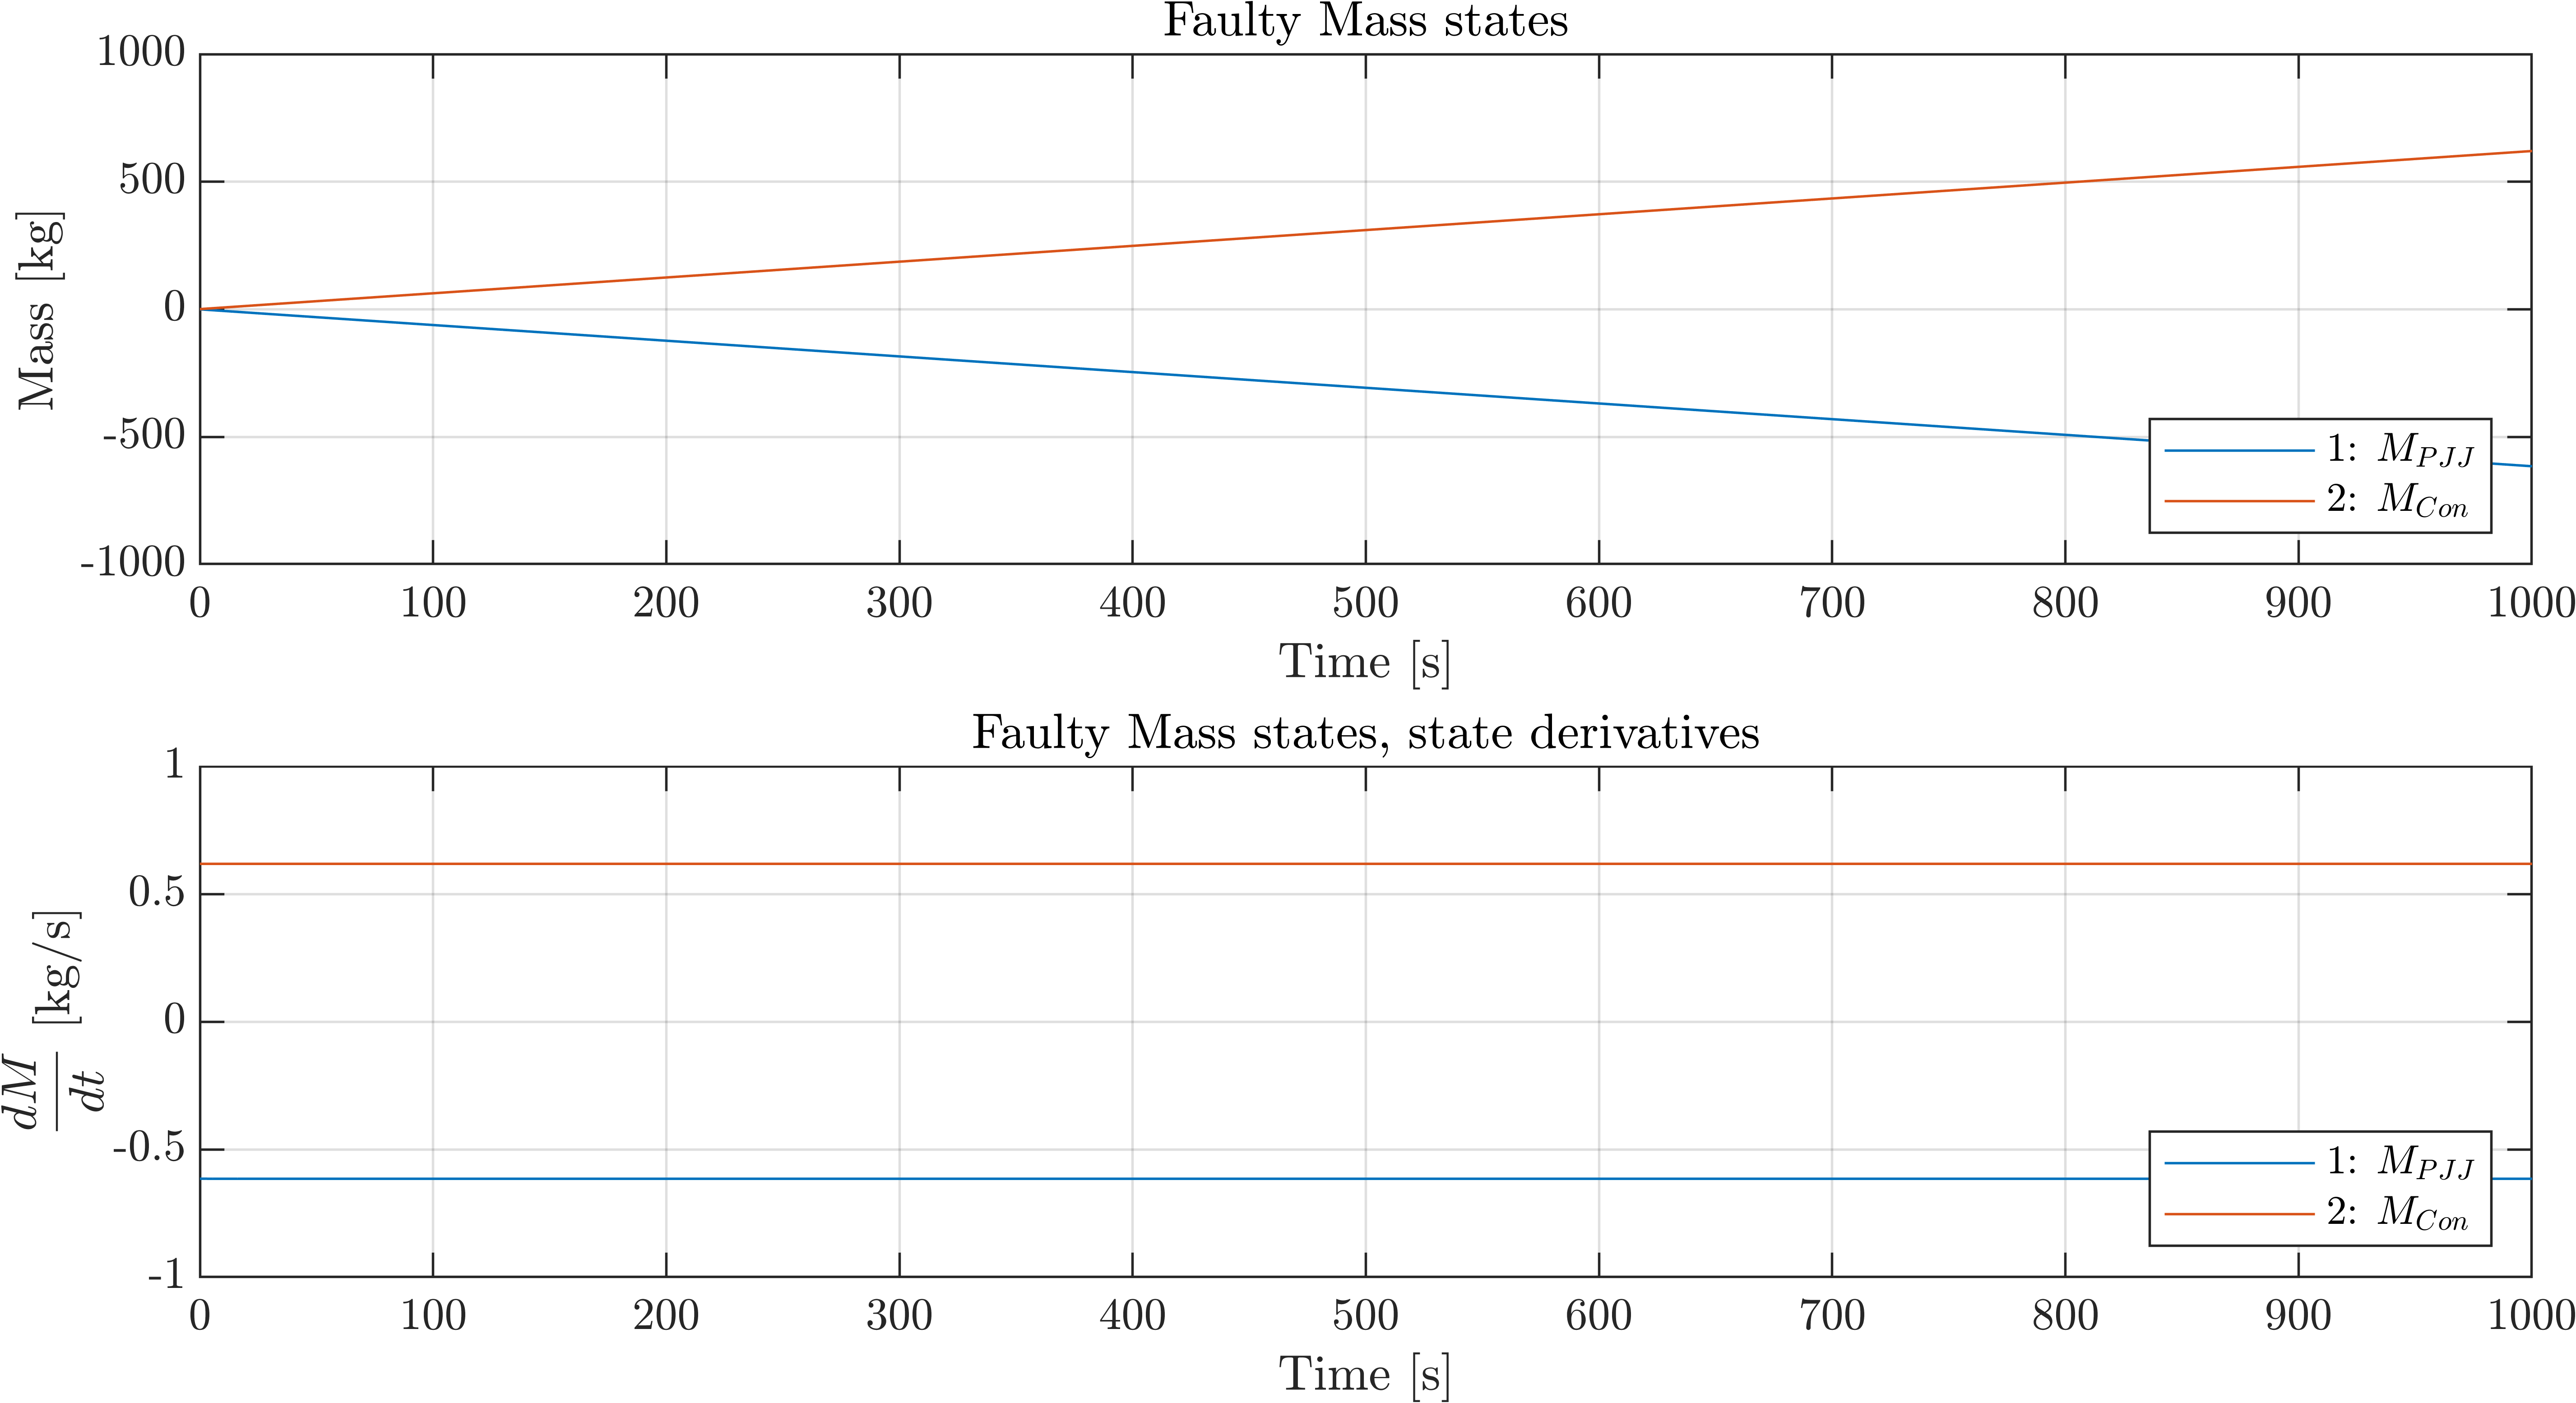
\includegraphics[width=0.9\textwidth]{../Graphics/nonlin_sim_faulty_Mass.png}
		\label{fig:non_lin_sim_faulty_Mass}
	\end{figure}
\end{frame}




%%%%%%%%%%%%%%%%%

\begin{frame}{Modelling}{Verification: $M_{lv}$, $M_{v}$ and $\dot{m}_{air}$}
	\begin{itemize}
		\item States plotted: $M_{lv}$, $M_v$ and $\dot{m}_{air}$
		\item Mass of vapour inside evaporator $M_v$ has constant non-zero derivative at SS
		\item Considered numeric error and mitigated by subtracting function of compressor speed
	\end{itemize}
	\begin{figure}[h]
		\centering
		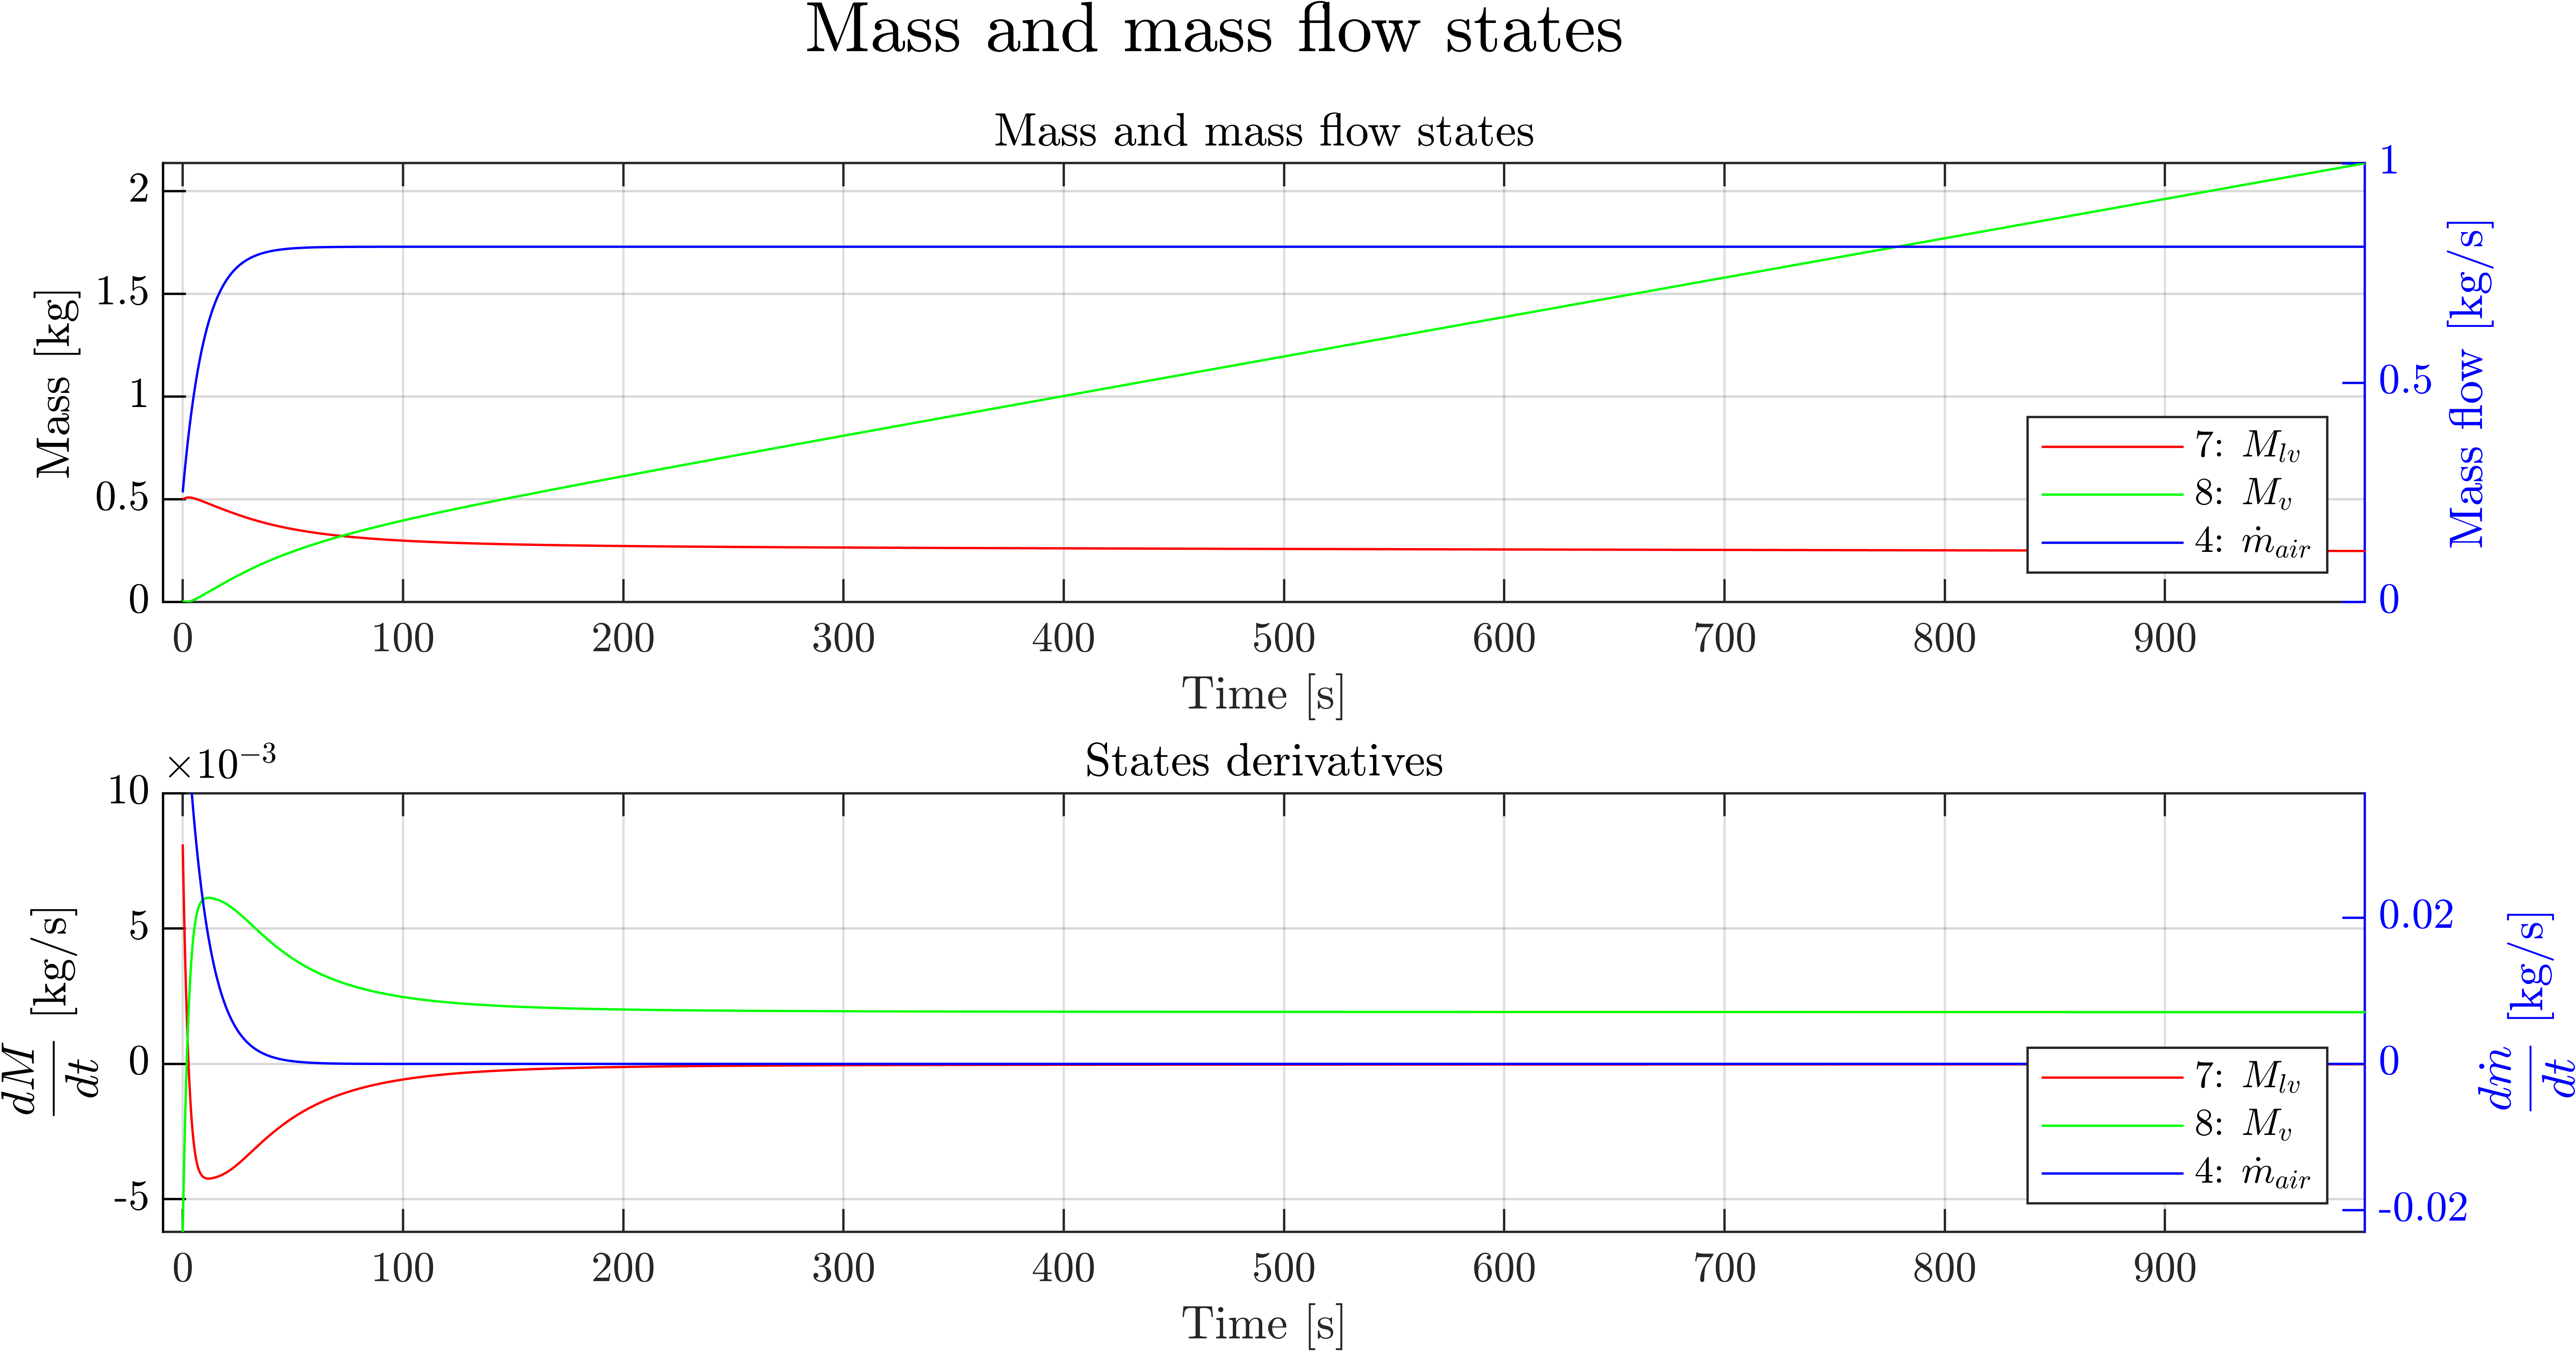
\includegraphics[width=1\textwidth]{../Graphics/nonlin_sim_Mass_Mvfucked.png}
		\caption{Notice two y-axis}
		\label{fig:non_lin_sim_Mass_Mvfucked}
		
	\end{figure}
	
\end{frame}



%%%%%%%%%%%%%%%%%

\begin{frame}{Modelling}{Verification: Discussion}
	\begin{itemize}
		\item Likely cause of errors: Simplifications in modelling section
		\begin{itemize}
			\item Pressure inside components not defined as states
			\item Results in mass inside components not affecting pressure and thereby flow through component
		\end{itemize}
	\end{itemize}

\end{frame}



%%%%%%%%%%%%%%%%%

\begin{frame}{Modelling}{Linearisation}
	\begin{itemize}
		\item Motivation: Non-linear model is not directly applicable for control strategy 
		\item Linearisation is thus performed at relevant OP
	\end{itemize}
	Non-linear model is transformed to the following form:
	\begin{equation} \label{eq:state_space}
		\begin{split}
			\dot{x} & = Ax + Bu + B_dd \\
			y 		& = Cx
		\end{split}
	\end{equation}
	by using the first order taylor expansion:
	\begin{equation}
		f(x) \approx f(x_o) + \left. \dfrac{\partial f}{\partial x} \right |_{x_o} \cdot (x-x_0)		
	\end{equation}
	where $f(x)$ = $\dot{x}$ and $x = (x, u, d)$.


\end{frame}



%%%%%%%%%%%%%%%%%

%\begin{frame}{Modelling}{Linearisation}
%	Resulting full taylor expansion expression:
%	\begin{equation} \label{eq:taylor}
%		\begin{split}
%			\dot{x}   \approx   f(x_o, u_o, d_o)   & +
%			\left. \dfrac{\partial f}{\partial x} \right |_{x_o, u_o, d_o} \cdot (x-x_0)  + 
%			\left. \dfrac{\partial f}{\partial u} \right |_{x_o, u_o, d_o} \cdot (u-u_0) \\ & +
%			\left. \dfrac{\partial f}{\partial d} \right |_{x_o, u_o, d_o} \cdot (d-d_0)
%		\end{split}
%	\end{equation}
%	With each partial derivative yielding a Jacobian on the form:
%	\begin{equation} \label{eq:jacobians}
%		\dfrac{\partial f}{\partial x} =
%		\begin{bmatrix}
%			\dfrac{\partial f_1}{\partial x_1} & \cdots & \dfrac{\partial f_1}{\partial x_{nx}} & \\
%			\vdots & \ddots & \vdots & \\
%			\dfrac{\partial f_e}{\partial x_1} & \cdots & \dfrac{\partial f_e}{\partial x_{nx}} &
%		\end{bmatrix}
%	\end{equation}
%	Where derivatives are made with respect to both states, inputs and disturbance $(x,u,d)$
%	
%
%\end{frame}
%
%
%
%%%%%%%%%%%%%%%%%%
%
%\begin{frame}{Modelling}{}
%	Resultingly the system matrix, input and disturbance input matrices are:
%	\begin{equation}
%		\left. \dfrac{\partial f}{\partial x} \right |_{x_o, u_o, d_o} = A, \;\;
%		\left. \dfrac{\partial f}{\partial u} \right |_{x_o, u_o, d_o} = B, \;\;
%		\left. \dfrac{\partial f}{\partial d} \right |_{x_o, u_o, d_o} = B_d
%	\end{equation}
%	Notes regarding operating point:
%	\begin{itemize}
%		\item Should be at equilibrium
%		\item If not then some eigenvalues of $A$ will have zero real parts. 
%		\item In this case not all dynamics of the system are captured at that operating point (Hartman-Grobman theorem)
%	\end{itemize}
%\end{frame}



%%%%%%%%%%%%%%%%%

\begin{frame}{Modelling}{Linearisation: B matrix}
	\begin{itemize}
		\item Chosen operating point from Hi-Fi simulation is at SS with $T_{air} = -5 ^{\circ} C$
		\item Resulting B matrix shows two inputs not mapping to states. These are simply removed.
	\end{itemize}
\begin{align}
	B = &\kbordermatrix{
		& \omega & \Theta_{eva} & \Theta_{con} & U_{fan\_con} & U_{fan\_eva} \\
		T_m 			& 0 & 0 & 0 & -0.0093 & 0\\
		\dot{m}_{air}	& 0 & 0 & 0 & 0 & \text{7.9630e-04}\\
		T_{mlv}			& 0 & 0 & 0 & 0 & 0\\
		T_{mv}			& 0 & 0 & 0 & 0 & 0.0011\\
		M_{lv}			& 0 & \text{5.0703e-04} & 0 & 0 & 0\\
		M_v 			& 0 & 0 & 0 & 0 & 0\\
		T_{air}  		& 0 & 0 & 0 & 0 & \text{1.0069e-04}\\
		T_{box}	 		& 0 & 0 & 0 & 0 & 0\\
		T_{cargo} 		& 0 & 0 & 0 & 0 & 0\\
		T_v 			& 0 & 0 & 0 & 0 & 0
	} \label{eq:B_full}
\end{align}
\end{frame}



%%%%%%%%%%%%%%%%%

\begin{frame}{Modelling}{Linearisation: Discussion}
	\begin{itemize}
		\item $\omega$ and $\Theta_2$ do not map to any states
		\begin{itemize}
			\item Explanation: Too simple model - several components do not connect
			\item Example: No flow coupling between $\dot{m}_{in}$ and $\dot{m}_{out}$ of condenser.
			\begin{itemize}
				\item Result: No control of flow into evaporator
			\end{itemize}
		\end{itemize}
		\item $A$ matrix is stable
		\item One pole is -1.3e-9 indicating a zero pole
		\begin{itemize}
			\item Inferred: Not all dynamics are captured by the chosen operating point
		\end{itemize}
	\end{itemize}
\end{frame}



%%%%%%%%%%%%%%%%%

\begin{frame}{Modelling}{Controllability and Observability}
	\textbf{Controllability}
	\begin{itemize}
		\item Checked to ensure that all inputs map to states
		\item Controllability matrix should be full rank:
	\end{itemize}
	\begin{equation} \label{eq:ctrb}
		Q_c = [A|B] = \begin{bmatrix}  B & AB & \cdots & A^{n-1}B  \end{bmatrix}
	\end{equation}

	\textbf{Observability}
	\begin{itemize}
		\item Checked to ensure that all states map to outputs
		\item Observability matrix should be full rank:
	\end{itemize}
	\begin{equation}
		Q_o = [A|C] = \begin{bmatrix}
			C \\ CA \\ \vdots \\ CA^{n-1}
		\end{bmatrix}
	\end{equation}
\end{frame}



%%%%%%%%%%%%%%%%%

\begin{frame}{Modelling}{Controllability and Observability: Results}
	\begin{itemize}
		\item Controllability matrix has full rank: Rank of [A|B] = 10
		\item Observability matrix has \underline{not} full rank: Rank of [A|C] = 8
			\begin{itemize}
				\item Actions are taken to mitigate: Kalman decomposition for unobservable system
				\item Two states are not observable: 
				\begin{itemize}
					\item Condenser metal temperature: $T_m$
					\item Evaporator vapour CV mass: $M_v$
				\end{itemize} 
			\end{itemize}
		
	\end{itemize}
\end{frame}



%%%%%%%%%%%%%%%%%

\begin{frame}{Modelling}{Kalman decomposition for unobservable system}
	\begin{itemize}
		\item Used to obtain an observable subsystem
	\end{itemize}
	For the Kalman decomposition, there exists a nonsingular P  $\in \mathbb{R} ^{n x n}$ such that
	\begin{equation}
		PAP^{-1} = \begin{bmatrix}
			A_{11}       & 0 \\
			A_{21}       & A_{22} \\
		\end{bmatrix}
	\end{equation}
	
	and
	
	\begin{equation}
		CP^{-1} = \begin{bmatrix}
			C_{1}       & 0 \\
		\end{bmatrix}
	\end{equation}
	
	where $A_{11} \in \mathbb{R} ^{l x l}$ and $C_{1} \in \mathbb{R} ^{p x l}$, where p is the number of outputs and l is the number of observable states.
	
	Input and disturbance matrices are transformed as such:
	\begin{equation}
		PB = \begin{bmatrix}
			B_1 \\
			B_2
		\end{bmatrix}, \
		PB_d = \begin{bmatrix}
			{B_d}_1 \\
			{B_d}_2
		\end{bmatrix}
	\end{equation}
\end{frame}



%%%%%%%%%%%%%%%%%

\begin{frame}{Modelling}{Kalman Decomposition reduced system}
	Resulting B matrix:
	\begin{align}
		B_1 & = \kbordermatrix{
			& \omega & \Theta_{eva} & \Theta_{con} & U_{fan\_con} & U_{fan\_eva} \\
			\dot{m}_{air}	& 0 & 0 & 0 & 0 & 0.00083\\
			T_{mlv}			& 0 & 0 & 0 & 0 & 0\\
			T_{mv}			& 0 & 0 & 0 & 0 & 0.0011\\
			M_{lv}			& 0 & 0.0005 & 0 & 0 & 0\\
			T_{air}  		& 0 & 0 & 0 & 0 & 0.0001\\
			T_{box}	 		& 0 & 0 & 0 & 0 & 0\\
			T_{cargo} 		& 0 & 0 & 0 & 0 & 0\\
			T_v 			& 0 & 0 & 0 & 0 & 0
		} \label{eq:B1}
	\end{align}
	\begin{itemize}
		\item Another input $U_{fan\_con}$ does not map to states
		\item Is also removed
	\end{itemize}
\end{frame}



%%%%%%%%%%%%%%%%%

\begin{frame}{Modelling}{Condition number}
	\begin{itemize}
		\item Brings nuance to degree of controllability and observability
		\item "Large" condition numbers are generally undesirable
	\end{itemize}
	Definition:
	\begin{equation}
		\kappa (G(j\omega)) = \frac{\bar{\sigma}(G(j\omega))}{\underline{\sigma}(G(j\omega))}
	\end{equation}
	where $G(j\omega)$ is the transfer matrix of the system and
	\begin{itemize}
		\item $\bar{\sigma}$ is the largest singular value
		\item $\underline{\sigma}$ is the smallest singular value
	\end{itemize}
	Found from Singular Value Decomposition (SVD).
	
	\begin{itemize}
		\item Condition numbers for $Q_c$ are:
		\begin{itemize}
			\item 1.195e+9 for 'two state reduced' system 
			\item 2.934e+8 for Kalman decomposition reduced system
		\end{itemize}
	\end{itemize}
\end{frame}




\section{Controller}
\begin{frame}{Title}{Subtitle}
	 \textbf{Some text}
	 \begin{itemize}
	 	\item Item
	 \end{itemize}
\end{frame}

%%%%%%%%%%%%%%%%%

\begin{frame}{Next slide title}{Next slide subtitle}
	 \textbf{Some text}
	\begin{itemize}
		\item Item
	\end{itemize}
\end{frame}

%%%%%%%%%%%%%%%%%

\section{Robustness Analysis}
\begin{frame}{Title}{Subtitle}
	 \textbf{Some text}
	 \begin{itemize}
	 	\item Item
	 \end{itemize}
\end{frame}

%%%%%%%%%%%%%%%%%

\begin{frame}{Next slide title}{Next slide subtitle}
	 \textbf{Some text}
	\begin{itemize}
		\item Item
	\end{itemize}
\end{frame}

%%%%%%%%%%%%%%%%%

\section{Test - Controller with Linear Model}
\begin{frame}{Title}{Subtitle}
	 \textbf{Some text}
	 \begin{itemize}
	 	\item Item
	 \end{itemize}
\end{frame}

%%%%%%%%%%%%%%%%%

\begin{frame}{Next slide title}{Next slide subtitle}
	 \textbf{Some text}
	\begin{itemize}
		\item Item
	\end{itemize}
\end{frame}

%%%%%%%%%%%%%%%%%

\section{Test - Controller with Hi-Fi Model}
\begin{frame}{Test results}{HiFi model control}
	 \textbf{Test setup}
	 \begin{figure}[h!]
	 	\centering
	 	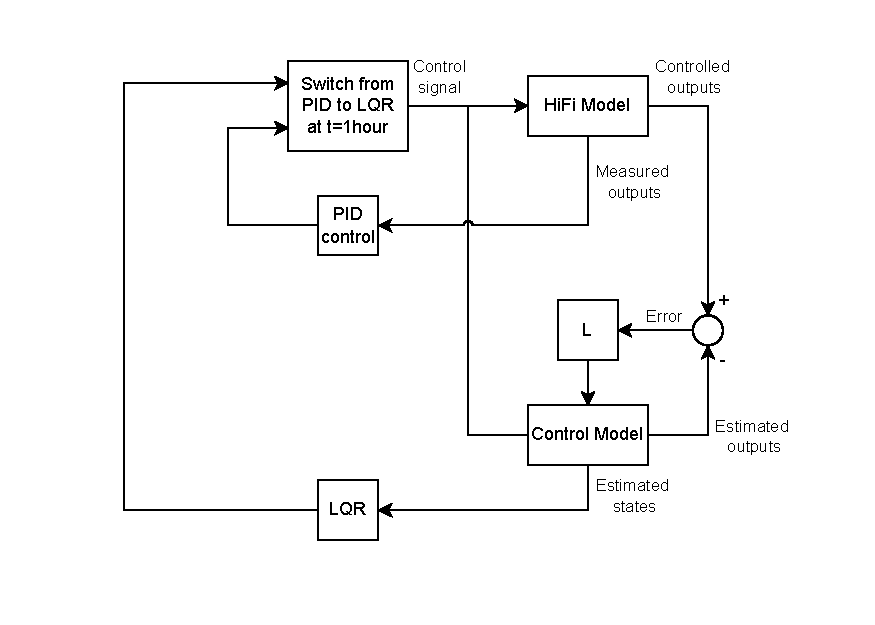
\includegraphics[width=0.8\textwidth]{../Graphics/HiFi_simulation_test_diagram.pdf}
	 	\label{fig:test_setup}
	 \end{figure}
 \begin{itemize}
 	\item No disturbance
 	\item Sine disturbance
 	\item Step disturbance
 \end{itemize}
\end{frame}

%%%%%%%%%%%%%%%%%

\begin{frame}{Test results}{HiFi model control}
	\textbf{No disturbance - controlled outputs}
	\begin{figure}[H]
		\centering
		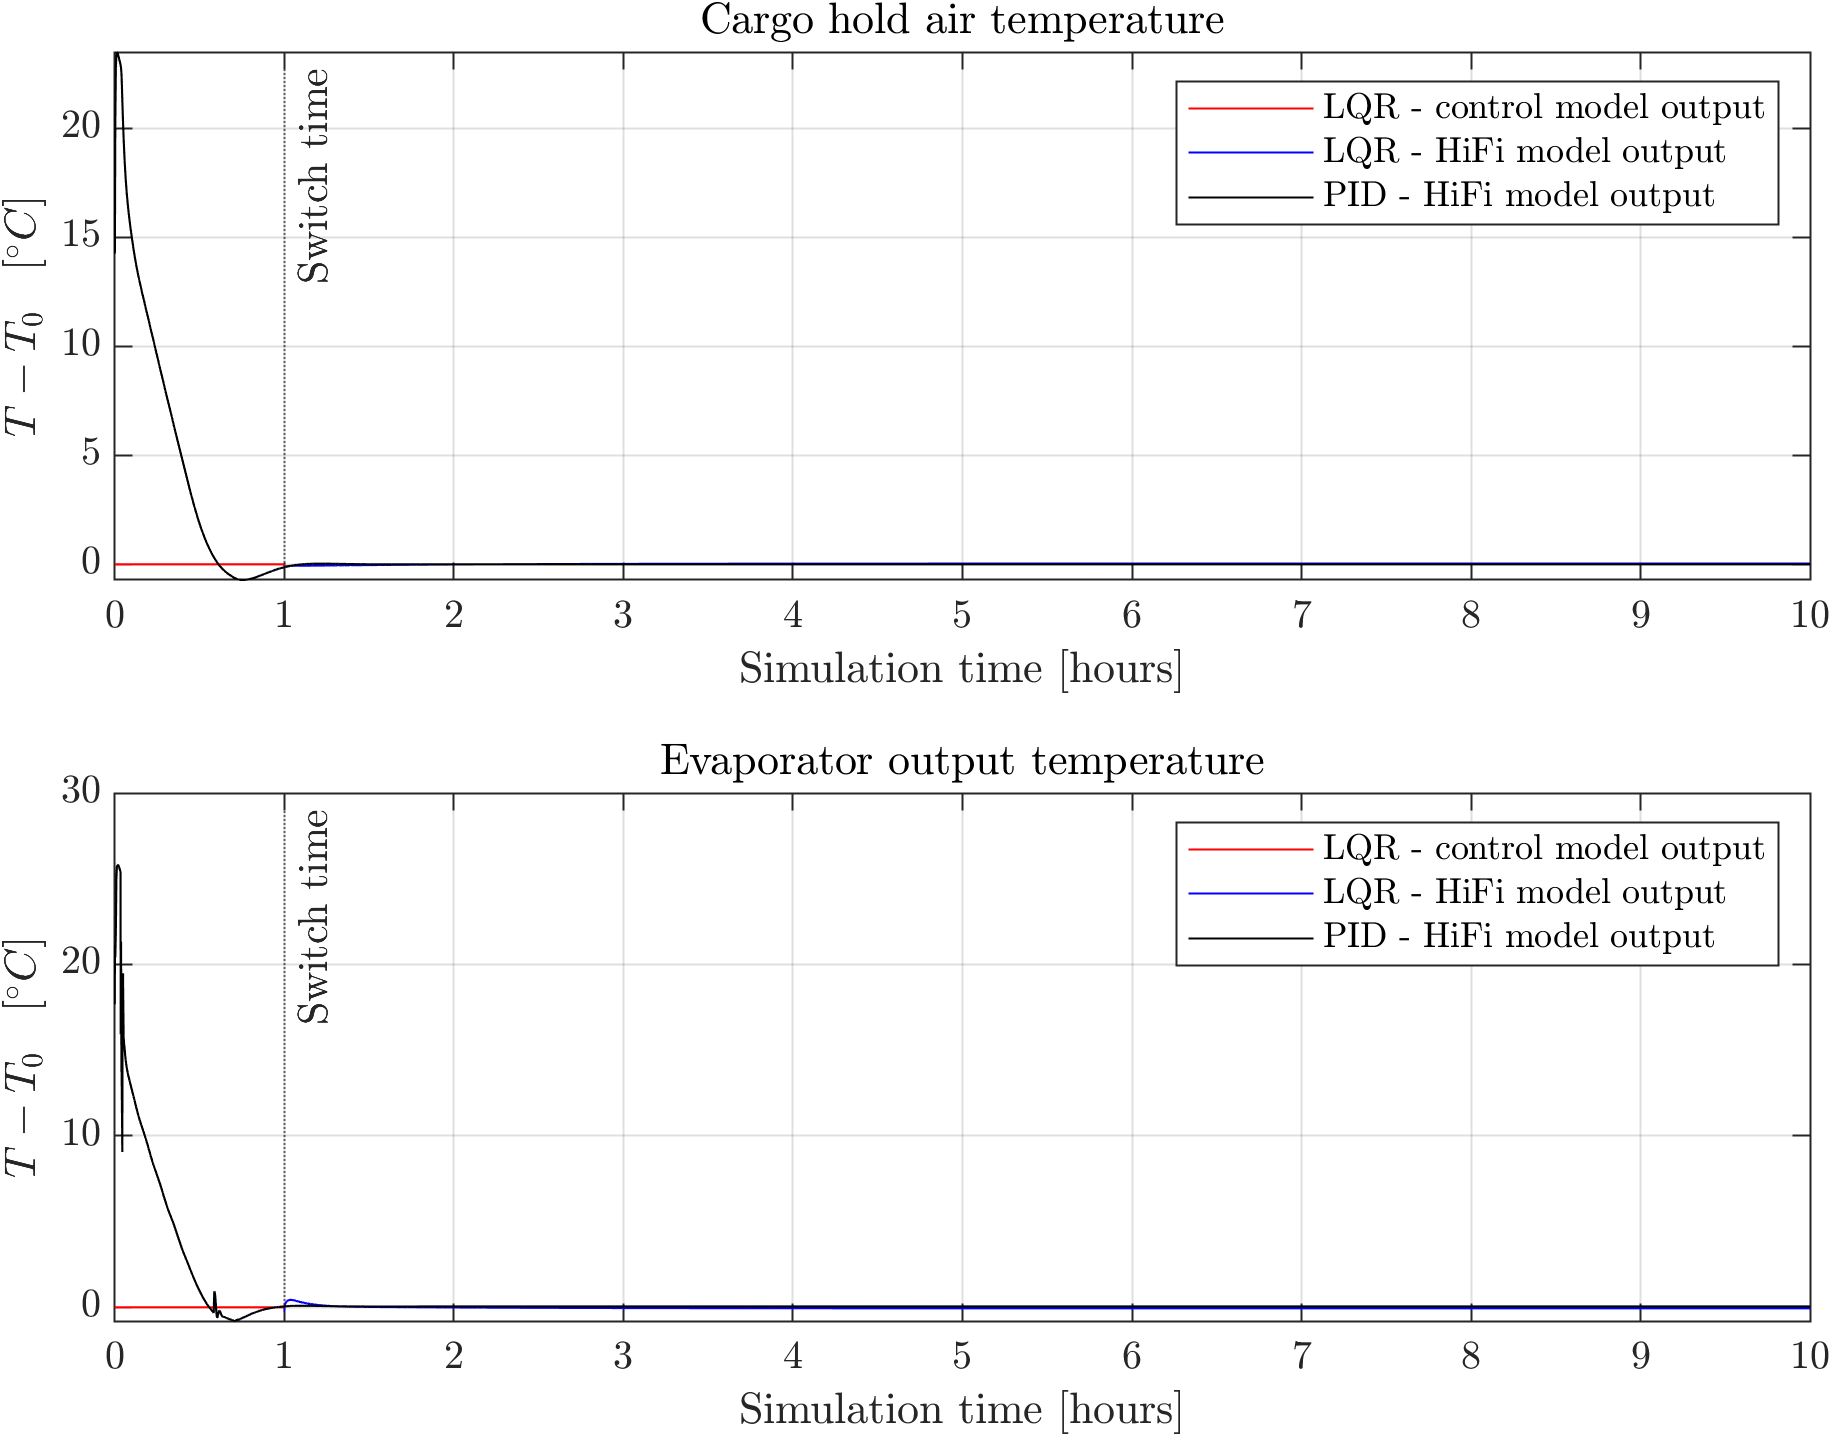
\includegraphics[width=0.8\textwidth]{../Graphics/fig_LQRvsKresten_noDist.png}
	\end{figure} 
\end{frame}

%%%%%%%%%%%%%%%%%

\begin{frame}{Test results}{HiFi model control}
	 \textbf{No disturbance - control signals}
	\begin{figure}[H]
		\centering
		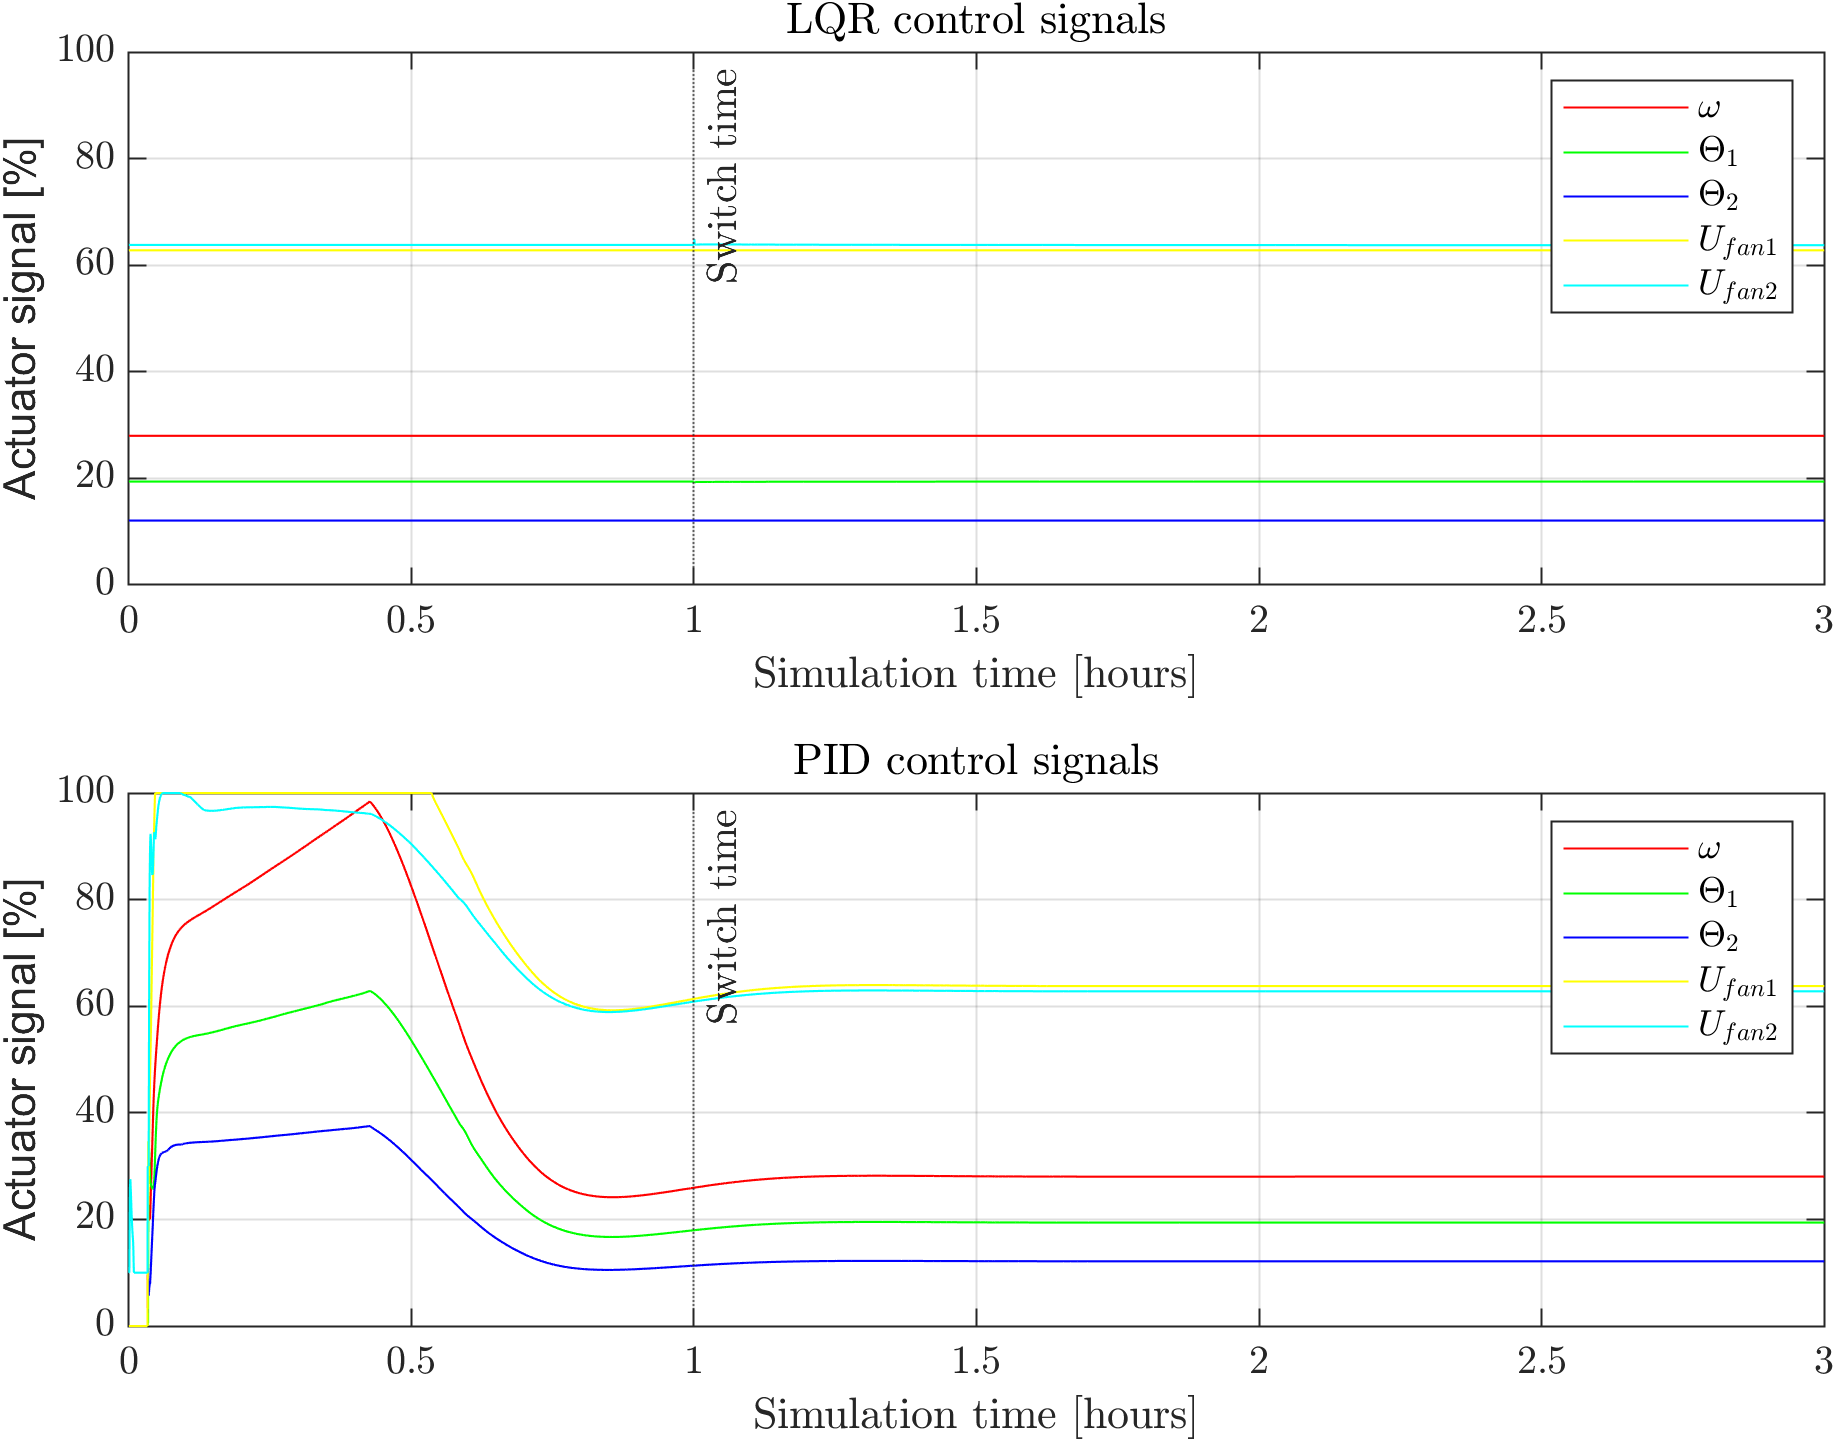
\includegraphics[width=0.8\textwidth]{../Graphics/fig_inputs_noDist.png}
	\end{figure}
\end{frame}

%%%%%%%%%%%%%%%%%

\begin{frame}{Test results}{HiFi model control}
	\textbf{Sine disturbance - controlled outputs}
	\begin{figure}[H]
		\centering
		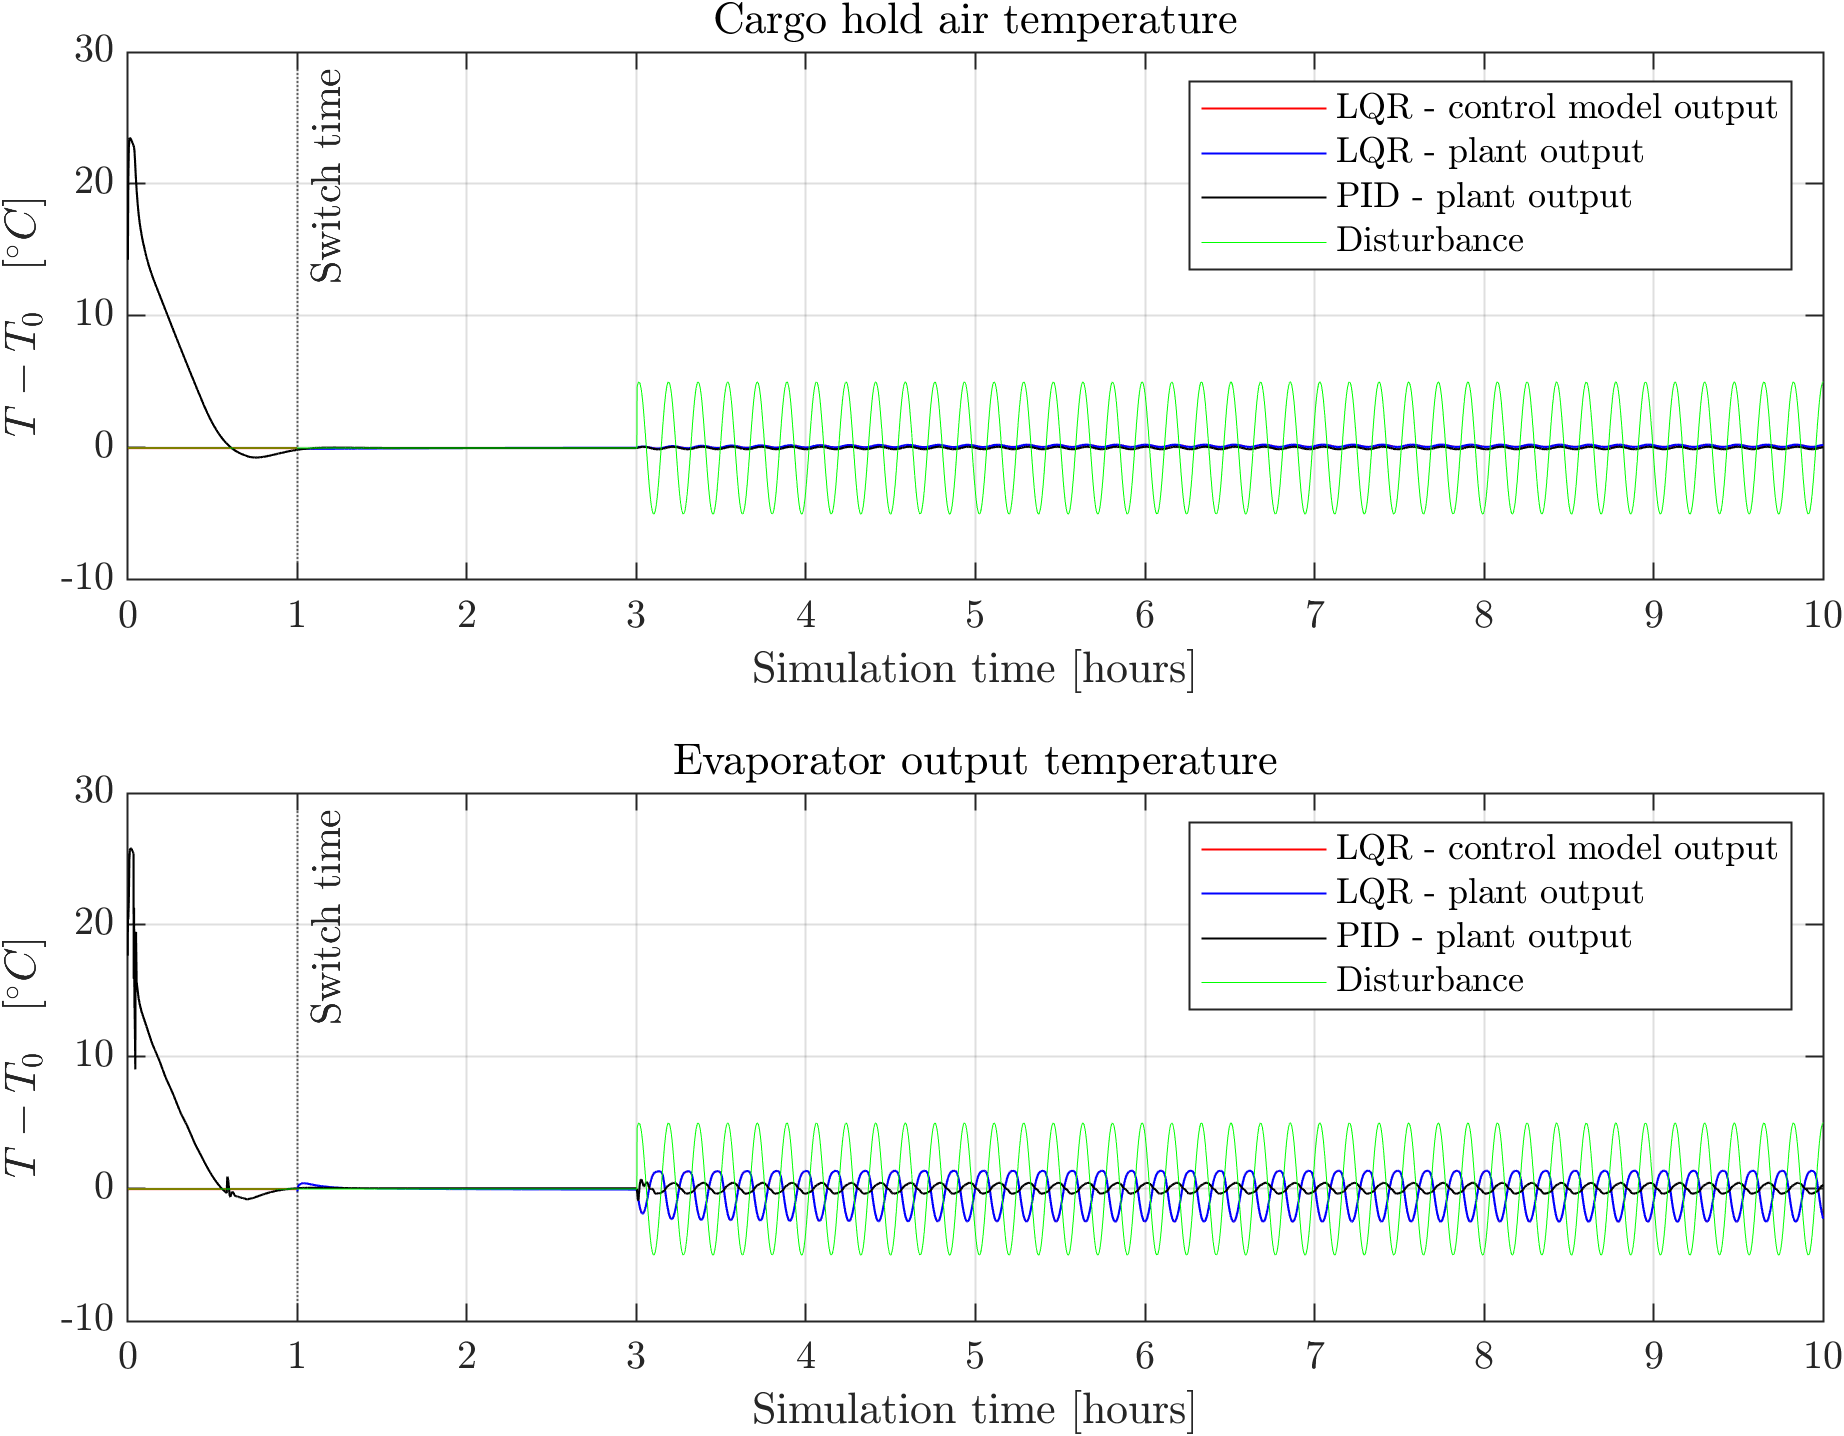
\includegraphics[width=0.8\textwidth]{../Graphics/fig_LQRvsKresten_sineDist.png}
	\end{figure} 
\end{frame}

%%%%%%%%%%%%%%%%%

\begin{frame}{Test results}{HiFi model control}
	\textbf{Sine disturbance - control signals}
	\begin{figure}[H]
		\centering
		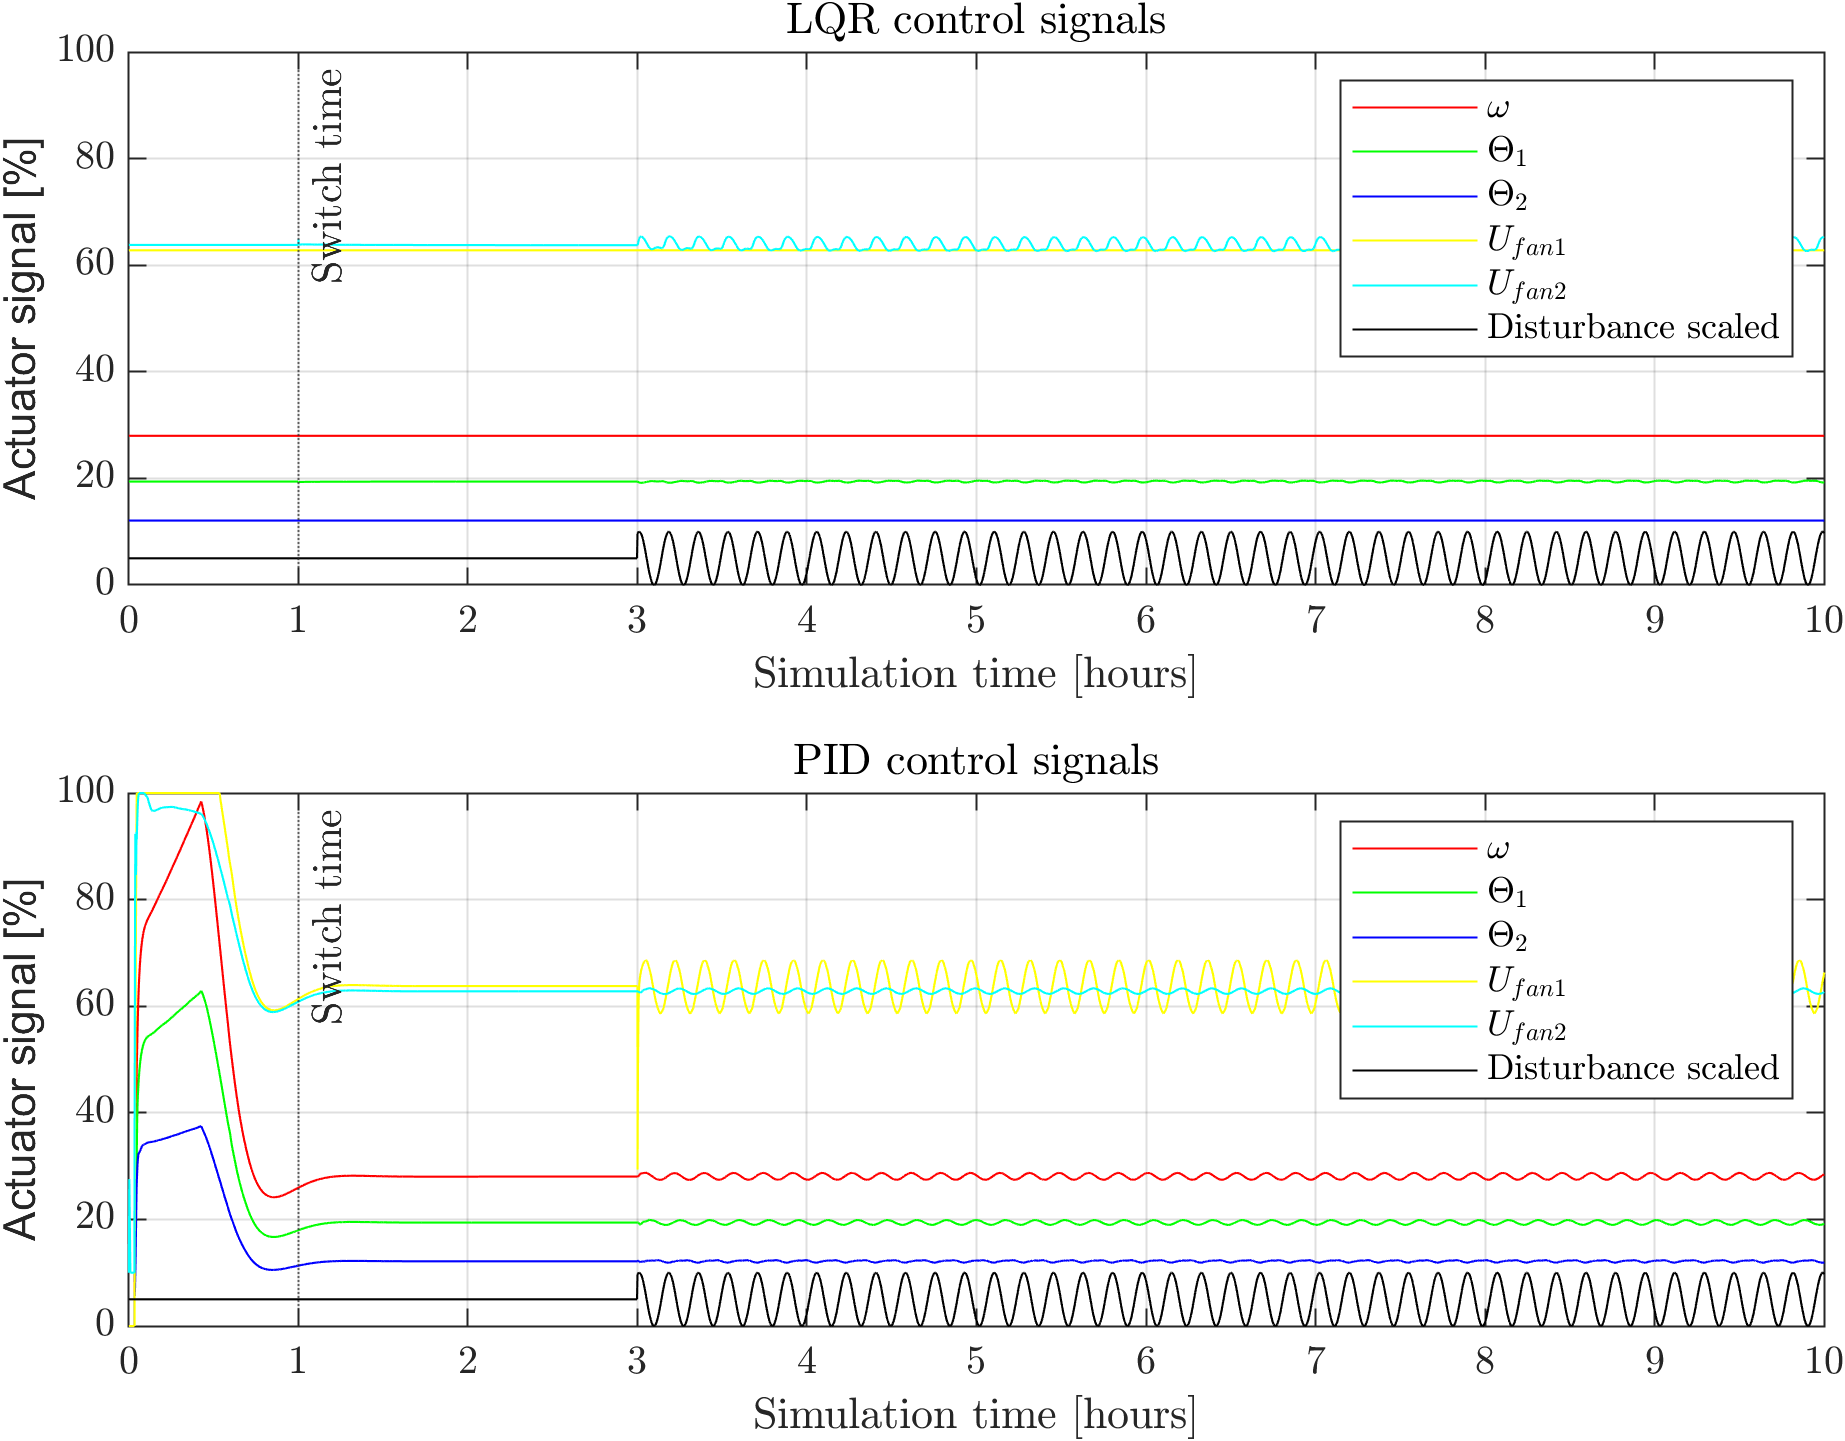
\includegraphics[width=0.8\textwidth]{../Graphics/fig_inputs_sineDist.png}
	\end{figure}
\end{frame}

%%%%%%%%%%%%%%%%%

\begin{frame}{Test results}{HiFi model control}
	\textbf{Step disturbance - controlled outputs}
	\begin{figure}[H]
		\centering
		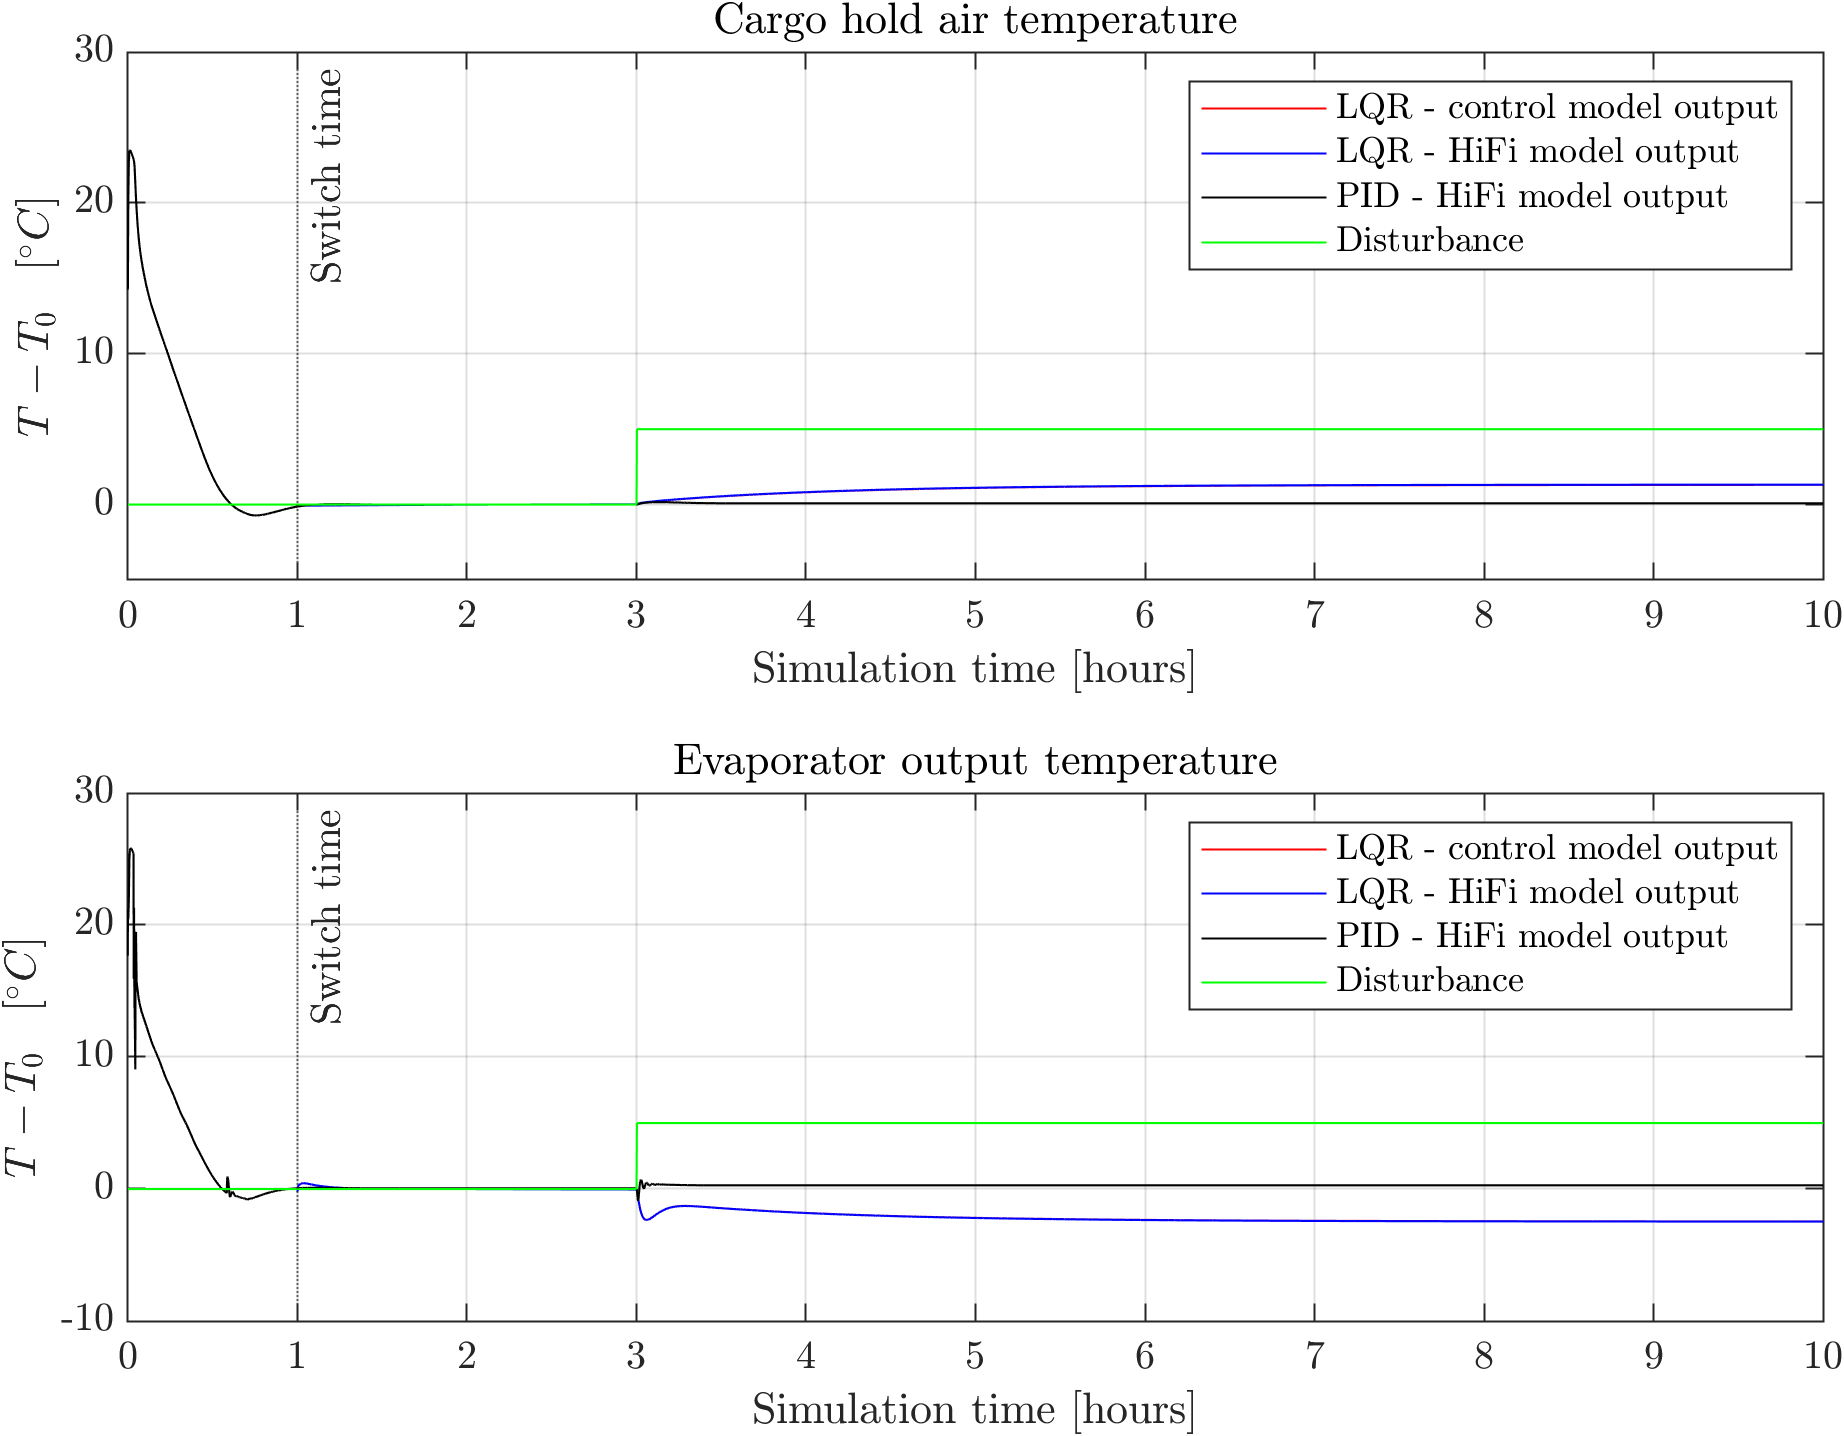
\includegraphics[width=0.8\textwidth]{../Graphics/fig_LQRvsKresten_stepDist.png}
	\end{figure} 
\end{frame}

%%%%%%%%%%%%%%%%%

\begin{frame}{Test results}{HiFi model control}
	\textbf{Step disturbance - control signals}
	\begin{figure}[H]
		\centering
		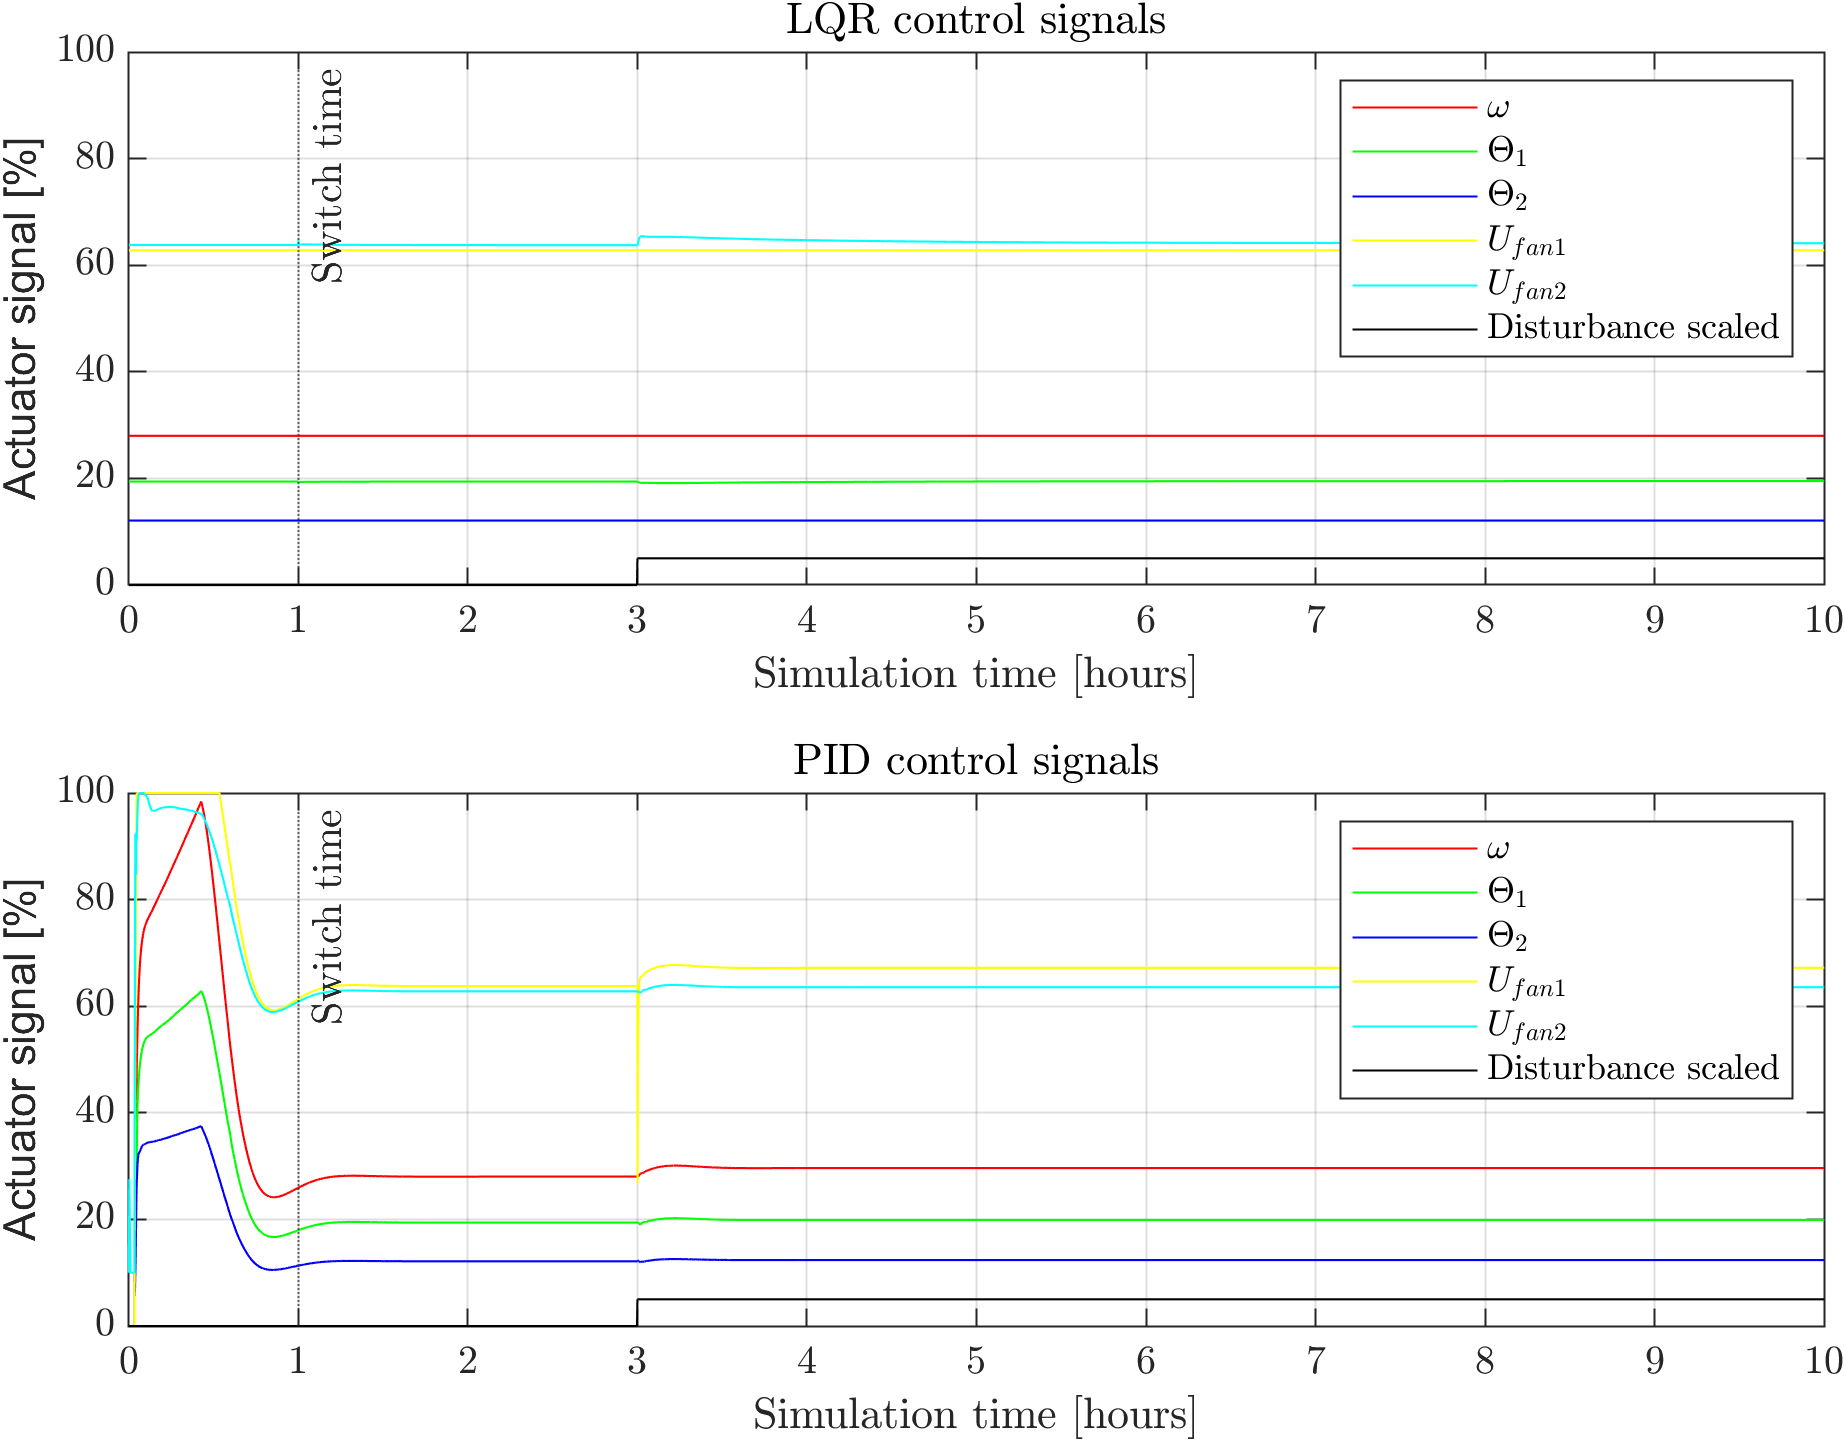
\includegraphics[width=0.8\textwidth]{../Graphics/fig_inputs_stepDist.png}
	\end{figure}
\end{frame}

%%%%%%%%%%%%%%%%%





\section{Conclusion}
\begin{frame}{Title}{Subtitle}
	 \textbf{Some text}
	 \begin{itemize}
	 	\item Item
	 \end{itemize}
\end{frame}

%%%%%%%%%%%%%%%%%

\begin{frame}{Next slide title}{Next slide subtitle}
	 \textbf{Some text}
	\begin{itemize}
		\item Item
	\end{itemize}
\end{frame}

%%%%%%%%%%%%%%%%%

\section{Future work and improvements}
\begin{frame}{Title}{Subtitle}
	 \textbf{Some text}
	 \begin{itemize}
	 	\item Item
	 \end{itemize}
\end{frame}

%%%%%%%%%%%%%%%%%

\begin{frame}{Next slide title}{Next slide subtitle}
	 \textbf{Some text}
	\begin{itemize}
		\item Item
	\end{itemize}
\end{frame}

%%%%%%%%%%%%%%%%%










% ======================================================================




%\section{References}
%\begin{frame}{References}
%	\bibliographystyle{ieeetran}
%	\bibliography{../../RefLib/CA7Projekt.bib}
%\end{frame}

{\aauwavesbg
\begin{frame}[plain,noframenumbering]
  \finalpage{Open for questions}
\end{frame}}
%%%%%%%%%%%%%%%%

\end{document}
